% Soubory musí být v kódování, které je nastaveno v příkazu \usepackage[...]{inputenc}

\documentclass[%        Základní nastavení
%  draft,    				  % Testovací překlad
  12pt,       				% Velikost základního písma je 12 bodů
  a4paper,    				% Formát papíru je A4
  oneside,      			% Jednostranný tisk
	%twoside,      			% Dvoustranný tisk (kapitoly a další důležité části tedy začínají na lichých stranách)
	unicode,						% Záložky a metainformace ve výsledném  PDF budou v kódování unicode
]{report}				    	% Dokument třídy 'zpráva', vhodná pro sazbu závěrečných prací s kapitolami

\usepackage[utf8]		  %	Kódování zdrojových souborů je UTF-8
	{inputenc}					% Balíček pro nastavení kódování zdrojových souborů

\usepackage[				% Nastavení geometrie stránky
	bindingoffset=10mm,		% Hřbet pro vazbu
	hmargin={25mm,25mm},	% Vnitřní a vnější okraj
	vmargin={25mm,34mm},	% Horní a dolní okraj
	footskip=17mm,			  % Velikost zápatí
	nohead,					      % Bez záhlaví
	marginparsep=2mm,		  % Vzdálenost marginálií
	marginparwidth=18mm,	% Šířka marginálií
]{geometry}
\usepackage{siunitx}
\usepackage{sectsty}
	%přetypuje nadpisy všech úrovní na bezpatkové, kromě \chapter, která je přenastavena zvlášť v thesis.sty
	\allsectionsfont{\sffamily}

\usepackage{graphicx} % Balíček 'graphicx' pro vkládání obrázků
											% Nutné pro vložení logotypů školy a fakulty

\usepackage[          % Balíček 'acronym' pro sazby zkratek a symbolů
	nohyperlinks				% Nebudou tvořeny hypertextové odkazy do seznamu zkratek
]{acronym}						
											% Nutné pro použití prostředí 'acronym' balíčku 'thesis'

\usepackage[
	breaklinks=true,		% Hypertextové odkazy mohou obsahovat zalomení řádku
	hypertexnames=false % Názvy hypertext. odkazů budou tvořeny nezávisle na názvech TeXu
]{hyperref}						% Balíček 'hyperref' pro sazbu hypertextových odkazů
											% Nutné pro použití příkazu 'pdfsettings' balíčku 'thesis'

\usepackage{pdfpages} % Balíček umožňující vkládat stránky z PDF souborů
                      % Nutné při vkládání titulních listů a zadání přímo
                      % ve formátu PDF z informačního systému

\usepackage{enumitem} % Balíček pro nastavení mezerování v odrážkách
  \setlist{topsep=0pt,partopsep=0pt,noitemsep} % konkrétní nastavení

\usepackage{cmap} 		% Balíček cmap zajišťuje, že PDF vytvořené `pdflatexem' je
											% plně "prohledávatelné" a "kopírovatelné"

%\usepackage{upgreek}	% Balíček pro sazbu stojatých řeckých písmem
											%% např. stojaté pí: \uppi
											%% např. stojaté mí: \upmu (použitelné třeba v mikrometrech)
											%% pozor, grafická nekompatibilita s fonty typu Computer Modern!
                      
%\usepackage{amsmath} %balíček pro sabu náročnější matematiky                 

\usepackage{dirtree}	% sazba adresářové struktury
                      % vhodné pro prezentaci obsahu elektronické přílohy (např. CD)

\usepackage[formats]{listings}	% Balíček pro sazbu zdrojových textů
\lstset{              % nastavení
%	Definice jazyka použitého ve výpisech
%    language=[LaTeX]{TeX},	% LaTeX
%	language={Matlab},		% Matlab
	language={C},           % jazyk C
    basicstyle=\ttfamily,	% definice základního stylu písma
    tabsize=2,			% definice velikosti tabulátoru
    inputencoding=utf8,         % pro soubory uložené v kódování UTF-8
		columns=fixed,  %fixed nebo flexible,
		fontadjust=true %licovani sloupcu
    extendedchars=true,
    literate=%  definice symbolů s diakritikou
    {á}{{\'a}}1
    {č}{{\v{c}}}1
    {ď}{{\v{d}}}1
    {é}{{\'e}}1
    {ě}{{\v{e}}}1
    {í}{{\'i}}1
    {ň}{{\v{n}}}1
    {ó}{{\'o}}1
    {ř}{{\v{r}}}1
    {š}{{\v{s}}}1
    {ť}{{\v{t}}}1
    {ú}{{\'u}}1
    {ů}{{\r{u}}}1
    {ý}{{\'y}}1
    {ž}{{\v{z}}}1
    {Á}{{\'A}}1
    {Č}{{\v{C}}}1
    {Ď}{{\v{D}}}1
    {É}{{\'E}}1
    {Ě}{{\v{E}}}1
    {Í}{{\'I}}1
    {Ň}{{\v{N}}}1
    {Ó}{{\'O}}1
    {Ř}{{\v{R}}}1
    {Š}{{\v{S}}}1
    {Ť}{{\v{T}}}1
    {Ú}{{\'U}}1
    {Ů}{{\r{U}}}1
    {Ý}{{\'Y}}1
    {Ž}{{\v{Z}}}1
}

%%%%%%%%%%%%%%%%%%%%%%%%%%%%%%%%%%%%%%%%%%%%%%%%%%%%%%%%%%%%%%%%%
%%%%%%      Definice informací o dokumentu             %%%%%%%%%%
%%%%%%%%%%%%%%%%%%%%%%%%%%%%%%%%%%%%%%%%%%%%%%%%%%%%%%%%%%%%%%%%%

% V tomto souboru se nastavují téměř veškeré informace, proměnné mezi studenty:
% jméno, název práce, pohlaví atd.
% Tento soubor je SDÍLENÝ mezi textem práce a prezentací k obhajobě -- netřeba něco nastavovat na dvou místech.
\usepackage{url}
\usepackage{makecell}
\usepackage[
%%% Z následujících voleb jazyka lze použít pouze jednu
  %czech-english,		% originální jazyk je čeština, překlad je anglicky (výchozí)
  %english-czech,	% originální jazyk je angličtina, překlad je česky
  %slovak-english,	% originální jazyk je slovenština, překlad je anglicky
  english-slovak,	% originální jazyk je angličtina, překlad je slovensky
%
%%% Z následujících voleb typu práce lze použít pouze jednu
  semestral,		  % semestrální práce (nesází se abstrakty, prohlášení, poděkování) (výchozí)
  %bachelor,			%	bakalářská práce
  %master,			  % diplomová práce
  %treatise,			% pojednání o disertační práci
  %doctoral,			% disertační práce
%
%%% Z následujících voleb zarovnání objektů lze použít pouze jednu
%  left,				  % rovnice a popisky plovoucích objektů budou zarovnány vlevo
	center,			    % rovnice a popisky plovoucích objektů budou zarovnány na střed (vychozi)
%
]{thesis}   % Balíček pro sazbu studentských prací

%%% Jméno a příjmení autora ve tvaru
%  [tituly před jménem]{Křestní}{Příjmení}[tituly za jménem]
% Pokud osoba nemá titul před/za jménem, smažte celý řetězec '[...]'
\author[Bc.]{Jakub}{Senčák}

%%% Identifikační číslo autora (VUT ID)
\butid{196504}

%%% Pohlaví autora/autorky
% (nepoužije se ve variantě english-czech ani english-slovak)
% Číselná hodnota: 1...žena, 0...muž
\gender{0}

%%% Jméno a příjmení vedoucího/školitele včetně titulů
%  [tituly před jménem]{Křestní}{Příjmení}[tituly za jménem]
% Pokud osoba nemá titul před/za jménem, smažte celý řetězec '[...]'
\advisor[Ing.]{Adrián}{Tomášov}

%%% Jméno a příjmení oponenta včetně titulů
%  [tituly před jménem]{Křestní}{Příjmení}[tituly za jménem]
% Pokud osoba nemá titul před/za jménem, smažte celý řetězec '[...]'
% Nastavení oponenta se uplatní pouze v prezentaci k obhajobě;
% v případě, že nechcete, aby se na titulním snímku prezentace zobrazoval oponent, pouze příkaz zakomentujte;
% u obhajoby semestrální práce se oponent nezobrazuje (jelikož neexistuje)
% U dizertační práce jsou typicky dva až tři oponenti. Pokud je chcete mít na titulním slajdu, prosím ručně odkomentujte a upravte jejich jména v definici "VUT title page" v souboru thesis.sty.
\opponent[doc.\ Ing.]{Jan}{Hajný}[Ph.D.]

%%% Název práce
%  Parametr ve složených závorkách {} je název v originálním jazyce,
%  parametr v hranatých závorkách [] je překlad (podle toho jaký je originální jazyk).
%  V případě, že název Vaší práce je dlouhý a nevleze se celý do zápatí prezentace, použijte příkaz
%  \def\insertshorttitle{Zkác.\ náz.\ práce}
%  kde jako parametr vyplníte zkrácený název. Pokud nechcete zkracovat název, budete muset předefinovat,
%  jak se vytváří patička slidu. Viz odkaz: https://bit.ly/3EJTp5A
\title[Distributed acoustic sensing system data analysis applied for perimeter protection]{Distributed acoustic sensing system data analysis applied for perimeter protection}

%%% Označení oboru studia
%  Parametr ve složených závorkách {} je název oboru v originálním jazyce,
%  parametr v hranatých závorkách [] je překlad
\specialization[Teleinformatics]{Teleinformatika}

%%% Označení ústavu
%  Parametr ve složených závorkách {} je název ústavu v originálním jazyce,
%  parametr v hranatých závorkách [] je překlad
%\department[Department of Control and Instrumentation]{Ústav automatizace a měřicí techniky}
%\department[Department of Biomedical Engineering]{Ústav biomedicínského inženýrství}
%\department[Department of Electrical Power Engineering]{Ústav elektroenergetiky}
%\department[Department of Electrical and Electronic Technology]{Ústav elektrotechnologie}
%\department[Department of Physics]{Ústav fyziky}
%\department[Department of Foreign Languages]{Ústav jazyků}
%\department[Department of Mathematics]{Ústav matematiky}
%\department[Department of Microelectronics]{Ústav mikroelektroniky}
%\department[Department of Radio Electronics]{Ústav radioelektroniky}
%\department[Department of Theoretical and Experimental Electrical Engineering]{Ústav teoretické a experimentální elektrotechniky}
\department[Department of Telecommunications]{Ústav telekomunikací}
%\department[Department of Power Electrical and Electronic Engineering]{Ústav výkonové elektrotechniky a elektroniky}

%%% Označení fakulty
%  Parametr ve složených závorkách {} je název fakulty v originálním jazyce,
%  parametr v hranatých závorkách [] je překlad
%\faculty[Faculty of Architecture]{Fakulta architektury}
\faculty[Faculty of Electrical Engineering and~Communication]{Fakulta elektrotechniky a~komunikačních technologií}
%\faculty[Faculty of Chemistry]{Fakulta chemická}
%\faculty[Faculty of Information Technology]{Fakulta informačních technologií}
%\faculty[Faculty of Business and Management]{Fakulta podnikatelská}
%\faculty[Faculty of Civil Engineering]{Fakulta stavební}
%\faculty[Faculty of Mechanical Engineering]{Fakulta strojního inženýrství}
%\faculty[Faculty of Fine Arts]{Fakulta výtvarných umění}
%
%Nastavení logotypu (v hranatych zavorkach zkracene logo, ve slozenych plne):
\facultylogo[logo/FEKT\_zkratka\_barevne\_PANTONE\_CZ]{logo/UTKO_color_PANTONE_CZ}

%%% Rok odevzdání práce
\graduateyear{2023}
%%% Akademický rok odevzdání práce
\academicyear{2022/23}

%%% Datum obhajoby (uplatní se pouze v prezentaci k obhajobě)
\date{11.\,12.\,2022} 

%%% Místo obhajoby
% Na titulních stránkách bude automaticky vysázeno VELKÝMI písmeny (pokud tyto stránky sází šablona)
\city{Brno}

%%% Abstrakt
\abstract[%
Překlad abstraktu
(v~angličtině, pokud je originálním jazykem čeština či slovenština; v~češtině či slovenštině, pokud je originálním jazykem angličtina)
]{%
Abstrakt práce v~originálním jazyce
}

%%% Klíčová slova
\keywrds[%
Překlad klíčových slov
(v~angličtině, pokud je originálním jazykem čeština či slovenština; v~češtině či slovenštině, pokud je originálním jazykem angličtina)
]{%
Klíčová slova v~originálním jazyce
}

%%% Poděkování
\acknowledgement{%
I would like to thank my supervisor Ing.~Adrián Tomášov for leading me during my struggles with this work, for his time during our consultations and lots of patience. 
}%  % do tohoto souboru doplňte údaje o sobě, druhu práce, názvu...

%%%%%%%%%%%%%%%%%%%%%%%%%%%%%%%%%%%%%%%%%%%%%%%%%%%%%%%%%%%%%%%%%%%%%%%%

%%%%%%%%%%%%%%%%%%%%%%%%%%%%%%%%%%%%%%%%%%%%%%%%%%%%%%%%%%%%%%%%%%%%%%%%
%%%%%%     Nastavení polí ve Vlastnostech dokumentu PDF      %%%%%%%%%%%
%%%%%%%%%%%%%%%%%%%%%%%%%%%%%%%%%%%%%%%%%%%%%%%%%%%%%%%%%%%%%%%%%%%%%%%%
%% Při načteném balíčku 'hyperref' lze použít příkaz '\pdfsettings':
\pdfsettings
%  Nastavení polí je možné provést také ručně příkazem:
%\hypersetup{
%  pdftitle={Název studentské práce},    	% Pole 'Document Title'
%  pdfauthor={Autor studenstké práce},   	% Pole 'Author'
%  pdfsubject={Typ práce}, 						  	% Pole 'Subject'
%  pdfkeywords={Klíčová slova}           	% Pole 'Keywords'
%}
%%%%%%%%%%%%%%%%%%%%%%%%%%%%%%%%%%%%%%%%%%%%%%%%%%%%%%%%%%%%%%%%%%%%%%%

\pdfmapfile{=vafle.map}

%%%%%%%%%%%%%%%%%%%%%%%%%%%%%%%%%%%%%%%%%%%%%%%%%%%%%%%%%%%%%%%%%%%%%%%
%%%%%%%%%%%       Začátek dokumentu               %%%%%%%%%%%%%%%%%%%%%
%%%%%%%%%%%%%%%%%%%%%%%%%%%%%%%%%%%%%%%%%%%%%%%%%%%%%%%%%%%%%%%%%%%%%%%
\begin{document}
\pagestyle{empty} %vypnutí číslování stránek

%%% Vložení desek -- od září 2021 na žádost fakulty nepoužíváno
%\includepdf[pages=1]%  buďto generovaných informačním systémem
  %{pdf/student-desky}% název souboru nesmí obsahovat mezery!
%%% NEBO vytvoření desek z balíčku
%%\makecover
%%%
%\oddpage % při dvojstranném tisku přidá prázdnou stránku
%% kazdopádně ale:
%\setcounter{page}{1} %resetovaní čítače stránek -- desky do číslování nezahrnujeme

%% Vložení titulního listu
\includepdf[pages=1]%    buďto generovaného informačním systémem
  {pdf/student-titulka.pdf}% název souboru nesmí obsahovat mezery!
%% NEBO vytvoření titulní sƒtránky z balíčku
% \maketitle
%%
\oddpage  % při dvojstranném tisku se přidá prázdná stránka
   
%% Vložení zadání
\includepdf[pages=1]%   buďto generovaného informačním systémem
  {pdf/zadani.pdf}% název souboru nesmí obsahovat mezery!
%% NEBO lze vytvořit prázdný list příkazem ze šablony
%\patternpage{}%
%	{\sffamily\Huge\centering ZDE VLOŽIT LIST ZADÁNÍ}%
%	{\sffamily\centering Z~důvodu správného číslování stránek}
%%
\oddpage% při dvojstranném tisku se přidá prázdná stránka

%% Vysázení stránky s abstraktem
% \makeabstract

% Vysázení stránky s rozšířeným abstraktem
% (pokud píšete práci v češtině či slovenštině, vložení rozšířeného abstraktu zrušte;
%  pro semestrální projekt také není potřeba rozšířený abstrakt uvádět)
% % Vysázení stránky s rozšířeným abstraktem
% (týká se pouze bc. a dp. prací psaných v angličtině, viz Směrnice rektora 72/2017)
\cleardoublepage
\noindent
{\large\sffamily\bfseries\MakeUppercase{Rozšířený abstrakt}}
\\
Výtah ze směrnice rektora 72/2017:\\
\emph{Bakalářská a diplomová práce předložená v angličtině musí obsahovat rozšířený abstrakt v češtině
nebo slovenštině (čl. 15). To se netýká studentů, kteří studují studijní program akreditovaný v
angličtině.}
(čl. 3, par. 7)\\
\emph{Nebude-li vnitřní normou stanoveno jinak, doporučuje se rozšířený abstrakt o rozsahu přibližně 3
normostrany, který bude obsahovat úvod, popis řešení a shrnutí a zhodnocení výsledků.}
(čl. 15, par. 5)

%%% Vysázení citace práce
\makecitation

%%% Vysázení prohlášení o samostatnosti
\makedeclaration

%%% Vysázení poděkování
\makeacknowledgement

%%% Vysázení obsahu
\tableofcontents

%%% Vysázení seznamu obrázků
% (vynechejte, pokud máte dva nebo méně obrázků)
\listoffigures

%%% Vysázení seznamu tabulek
% (vynechejte, pokud máte dvě nebo méně tabulek)
\listoftables

%%% Vysázení seznamu výpisů kódu
% (vynechejte, pokud máte dva nebo méně výpisů)
\lstlistoflistings

\cleardoublepage\pagestyle{plain}   % zapnutí číslování stránek

%Pro vkládání kapitol i příloh používejte raději \include než \input
%%% Vložení souboru 'text/uvod.tex' s úvodem
\chapter*{Introduction}
\phantomsection
\addcontentsline{toc}{chapter}{Introduction}

This work explains the topic of \acs{das} (\acl{das}), which uses optical fiber as a sensor array. Light pulses are sent from the light source through the fiber. The light is reflected and scattered on imperfections in the fiber and is reflected back to the light source where its properties are measured like changes in frequency and phase. If there is a strain on the fiber or the fiber is subjected to vibrations of any type, it is possible to interpret them as an audio signal or as some kind of movement. DAS is used for applications such as perimeter monitoring, earthquake detection and localization, traffic monitoring and incident detection and many more. One of the uses is possibility to hear interpret the data as a audio signal and use it as a microphone, which makes optical fiber a big security vulnerability. Especially dangerous is the fact that the attackers do not need access to the server room or the devices themselves, but can connect to the fiber anywhere. There is also the issue of detecting these kinds of attacks because DAS has no impact on existing communication on the fiber.

The main goal of this work is to implement an application that takes the data in HDF5 file format and converts it to WAV audio file format. The second goal is to design an application for displaying the data in an waterfall graph. The design includes study of existing technology and the study of technology capable of displaying the data in real time.


The first chapter explains how the DAS system works, methods of measuring the strain on the fiber. Important part is also study of the HDF5 file format and specially the output of the DAS system. The second chapter explains the implementation of HDF5 to WAV converter. Mainly the contents of the DAS output file and the data processing involved. The last chapter covers the software design of the waterfall graph visualization, all the requirements and the final solution.





% the capabilities it has in terms of security risks. 
% The goal of this 





% Úvod studentské práce, např\,\dots

% Nečíslovaná kapitola Úvod obsahuje \uv{seznámení} čtenáře s~problematikou práce.
% Typicky se zde uvádí:
% (a) do jaké tematické oblasti práce spadá, (b) co jsou hlavní cíle celé práce a (c) jakým způsobem jich bylo dosaženo.
% Úvod zpravidla nepřesahuje jednu stranu.
% Poslední odstavec Úvodu standardně představuje základní strukturu celého dokumentu.

% Tato práce se věnuje oblasti \acs{DSP} (\acl{DSP}), zejména jevům, které nastanou při nedodržení Nyquistovy podmínky pro \ac{symfvz}.%
% \footnote{Tato věta je pouze ukázkou použití příkazů pro sazbu zkratek.}

% Šablona je nastavena na \emph{dvoustranný tisk}.
% Nebuďte překvapeni, že ve vzniklém PDF jsou volné stránky.
% Je to proto, aby důležité stránky jako např.\ začátky kapitol začínaly po vytisknutí a svázání vždy na pravé straně.
% %
% Pokud máte nějaký závažný důvod sázet (a~zejména tisknout) jednostranně, nezapomeňte si přepnout volbu \texttt{twoside} na \texttt{oneside}!

% \begin{acronym}[DSP]
% \acro{DSP}% název je shodný se zkráceným tvarem
% {číslicové zpracování signálů}
% \acro{fvz}% název a zkrácený tvar jsou odlišné
% [\ensuremath{\var{f}_{\const{vz}}}]%
% 8
% {vzorkovací kmitočet}
% \acro{symDFT}%
% [\ensuremath{\mathcal{F}\left\{.\right\}}]%
% {provedení diskrétní Fourierovy transformace}
% \end{acronym}

% %%% Vložení souboru 'text/cile.tex' s úvodem
% \chapter*{Cíle práce}
\phantomsection
\addcontentsline{toc}{chapter}{Cíle práce}

Konkrétní specifikace cílů, které má autor v~práci vyřešit.
Tato kapitola je \emph{volitelná} -- pokud váš studijní program nevyžaduje zvláštní kapitolu s cíli,
cíle specifikujte v~rámci Úvodu.

%%% Vložení souboru 'text/reseni' s popisem řešení práce
% (rozdělte na více souborů či kapitol, pokud je vhodné)
\chapter{Theoretical introduction}


\section{Optical reflectometry}

Optical reflectometry is used for measurements of optical cables' properties; it is capable of detecting defects, joints, breaks, or other damage and their location on the wire. It is the basis for \ac{generalotdr} or \ac{ofdr} and other optical sensors such as \ac{das}. A~pulse of light is sent from the source, such as a light-emitting diode (LED) or a laser diode (LD). The light travels from the source through the optical fiber in pulses and is reflected from the other side of the wire, through connections, breaks, damage, or imperfections in the material. All of these create some backscattering toward the light source. Rayleigh, Brillouin, and Raman scattering are all different kinds of scattering happening in the fiber \cite{progress}. 

\subsection{OTDR}

\ac{otdr} is the most widely used method. When a strain is applied to the fiber, it causes phase-shift changes in the light signal. Provides high sensitivity, resolution, and high sampling rates in the frequency range between hertz and kilohertz. \ac{otdr} has limitations in measuring slowly changing effects and noise components.

% \subsection{(\acs{otdr})}   %\acl{otdr} 

% \acl{otdr} 

%https://www.flukenetworks.com/expertise/learn-about/otdr


\subsection{OFDR}

\ac{ofdr} analyzes interference of signal between the initial signal and the backscattered signal but focuses on the frequency scan. It requires a highly tunable laser diode as a~source of light. The signal given by \ac{ofdr} contains frequency information that can be processed with the Fourier transformation, and the output would be the position of the reflective elements along the fiber length. There are also other methods to measure light properties such as \textit{C-OFDR} - coherent version of OFDR using light with the frequency with linear dependency but having problems with high noise levels, and \textit{DSS} - Mandelstam-Brillouin \cite{kislov_das_newparadigm}.


\section{Distributed Acoustic Sensing}

Implementation of \ac{das} system is usually done by \ac{generalotdr}, \ac{ofdr}, or analysis of other light properties such as polarization and backscatter correlation. \ac{das} allows the measurement of thousands of points on an optical wire without the need to cut the wire or have multiple sensors distributed along the wire. The measurement mechanism is based on optical reflectometry the same as in DTS (distributed temperature sensing), which is a variant of \ac{generalotdr}. Measurement is based on the sending of pulses of light into the optical fiber. The fiber creates a small light scattering (e. g. Rayleigh scattering) in the glass that travels back to the sensing unit (on the same side as the light source), which can be interpreted on the basis of the time of arrival as position on the wire. Backscattering light from the optical fiber segment is detected at the light source and has changes in amplitude or phase, which means that the fiber wire segment is affected in some way. \ac{das} is used in a wide range of applications, from locating seismic activity, locating trains along the train tracks, as a~gyroscope or an accelerometer or even as a~microphone \cite{WangYu2017RDVM}, \cite{kislov_das_newparadigm}.

\ac{das} uses optical fiber since many sensors are capable of detecting vibrations along the fiber \cite{gabai}. These sensors allow for the measurement of acoustic properties (frequency, amplitude, and phase) \cite{WangYu2017RDVM}. 

There are two types of optical fiber sensors:
\begin{enumerate}
    \item Point - These sensors measure only at the location of the transducer
    \item Distributed - The sensing element is the optical wire and can measure at many points along the optical wire. One of the great benefits of this approach is the possibility of using existing telecommunication infrastructure to build the sensing network.
\end{enumerate}

% \subsection{Raleigh scattering}

% For a given optical frequency, sensors based on Raleigh scattering can detect the intensity, phase, and polarization of light.   
% %TODO

\section{iDAS}

The distributed acoustic sensor is a~new addition to distributed optical fiber sensors used in the energy industry and can be used in many applications, for example, in detecting seismic activity. iDAS (intelligent distributed acoustic sensor) is one type of DAS sensor. One of the applications of this sensor is to record an acoustic signal. To determine the signal fidelity, a certain part of the wire is subjected to a known signal, e.g. sine wave. A measurement is made, and the result is compared with the existing recording device. The result suggests that iDAS has very good signal properties. The measured signal shows that almost no measurable crosstalk is exhibited between the two sensing channels on the wire.

The maximum sampling rate can be calculated from the speed of light that travels in glass at a speed of about \qty{200000}{\km/\s} which corresponds to approximately \qty{10}{\kHz} for \qty{10}{\km} long wire \cite{WangYu2017RDVM}.

% 10 kHz == 10 km, 1 kHz == 100 km [doplnit vzorcek]

\begin{itemize}
    \item Acoustic bandwidth
    \item Dynamic range - \qty{120}{\dB} as reported in \cite{dasseismic}
    \item Spatial resolution - about \qty{1}{\m} to \qty{10}{\m}, but up to \qty{25}{\cm} is possible
    \item Measurement range - The fiber length can be anywhere from a few hundred meters to more than \qty{100}{\km}.
\end{itemize}



\section{OptaSense ODH-F}

Data used in this project were obtained from \textit{OptaSense ODHF Distributed Acoustic Sensing Interrogator}\footnote{\url{https://www.optasense.com/technology/odhf/}}. This device is capable of monitoring optical fiber up to \qty{50}{\km} long (in qualitative mode). It is used for in-well flow monitoring, pipeline integrity management, and border security. OptaSense comes with \textit{DxS Visualization Software} which is capable of analyzing and processing output data from the unit. It can show the signal spectrum in a waterfall graph and create analysis, process the signal using \ac{fft}, and extract data to \verb|.wav| format. It has the limitation that it can only run in the Windows ecosystem and is proprietary software, so scientists cannot really change how they work with the data or how it is displayed.


\subsection{HDF5 file format}

In this project, the output of the DAS system is in \ac{hdf}. Data from the \ac{das} sensor is collected on the server and saved in \ac{hdf} file. \ac{hdf} creates a model for managing and storing data. The HDF Group\footnote{\url{https://www.hdfgroup.org/}} is the maintainer of the software package. Specifically, the \ac{hdf} format is used to store data, but it is only one of the three parts that make up the \ac{hdf} model. Parts of the \ac{hdf} model are:

\begin{itemize}
    \item File format - files ending with .h5
    \item Data model - specifies the building blocks of the \ac{hdf} file format
    \item Software - libraries, tools, APIs
\end{itemize}

\bigskip

\ac{hdf} data model has a folder-like organization, where the folders are called \textit{groups}. This model specifies the format in which the data are stored in the form of \ac{adm}, which specifies the organization of the data and the types of data. Every \ac{hdf} file has to have a~root group \textit{``/''}. Working with groups is very similar to directories on Linux systems; see Section \ref{dir:filestructure}. Each group can have \textit{datasets} that contain raw data, attributes, data types, and other objects. \ac{hdf} file can also specify links to other libraries and tools such as compression and filtering.

\bigskip
HSDF5 dataset has connections with other HDF5 objects:

\begin{itemize}
    \item \textbf{attributes} - named data object containing the name and the value
    \item \textbf{datatypes}:
    \begin{itemize}
        \item Atomic datatypes - time, string, integer, float.
        \item Composite datatypes - array, enumeration, compound, variable length.
    \end{itemize}
    \item \textbf{data} - data itself, for example, the result of measurement.
    \item \textbf{dataspace} - the shape of the data.
\end{itemize}


\begin{figure}
    \centering
    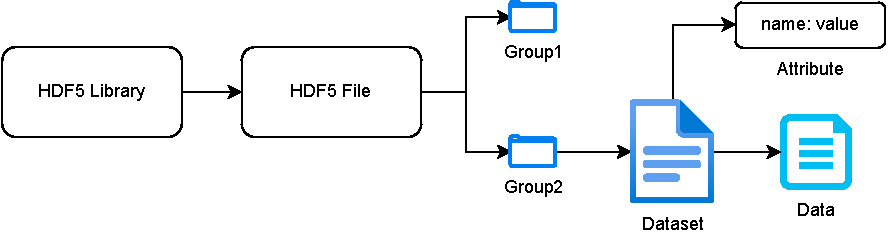
\includegraphics[width=\linewidth]{pdf/hdf5_file_structure.pdf}
    \caption{Basic HDF5 file structure}
    \label{fig:filestructure}
\end{figure}

\newpage %%%%%%%%%%%%%%%%%%%%%%%%%%%%%%%%%%%%%%%%%%%%%%%%%%%%%%%%%%%%%%%%%%%%%%%

\chapter{Implementation and software design}

\section{Program implementation of HDF5 to WAV}\label{lab:hdftowav}

The goal of this project is to create an application for reading data from the \ac{das} system and converting the data to the \verb|.wav| audio file format.

For the implementation of this application, the Python\footnote{\url{https://www.python.org/}} programming language was chosen. Python is a~great language for scientific use, data visualization, and graph plotting, which is the goal. The biggest advantage comes from the availability of scientific libraries. The opening of \verb |.h5| files is done with \verb|h5py| library\footnote{\url{https://www.h5py.org/}}. For working with dataset data types \verb|numpy|\footnote{\url{https://numpy.org/}} library is used. The function for interpolating arrays to a~certain range is also used \verb|interp|. Lastly, to convert the signal data to \verb|.wav| audio format \verb|scipy| library is used specifically \verb|io| module function \verb|wavfile|. To read all options and input arguments, the \verb|argparse| library is used\footnote{\url{https://docs.python.org/3/library/argparse.html}}.   

\subsection{Reading HDF5 file}\label{sec:readhdf}

The sample file recorded in the OptaSense ODH-F is in HDF5 file format. As \ac{hdf} files have a~user-defined structure on the application layer and in the binary form it is hard to say what is actually in the file. To better understand the contents of the \verb|.h5| file, \verb|h5dump| was performed and a conversion to JSON\footnote{\url{https://www.json.org/json-en.html}} was also performed by the \verb|h5tojson| program\footnote{\url{https://hdf5-json.readthedocs.io/en/latest/tools/h5json.html}}. The JSON file is quite large in size - the original HDF5 file is only \qty{52,7}{MB} and the JSON file is \qty{946,6}{MB}. The dump text file is half the size and provides the same information, but the datasets are harder to understand, but the whole file is only half the size of the JSON file at ``only'' \qty{420}{MB}. The JSON format is much easier to read. The structure of the file is divided into 3 parts:

\begin{itemize}
    \item \textit{apiVersion} - 1.1.1 version of API
    \item \textit{datasets} - Contain all the datasets organized by their UUID\footnote{Universally unique identifier} that are defined in the groups section. There is also an \textit{alias} that is in the format of a Unix-based system path, for example, \verb|"/Acquisition/Raw[0]/Custom/SampleCount"|. There are also other properties that define the shape and type of stored data. In this case, the properties are shown in the table \ref{tab:file_details}.
    \item \textit{groups} - Groups are named by a UUID. The group object has:
        \begin{itemize}
            \item \textit{alias} - Unix-like name; the first is root ``/'' group
            \item \textit{attributes} - define the type, name, and shape of the value of the attribute which is a string \verb|979bb2ac-99bf-4cb5-b410-5c16cd7872dc|
            \item \textit{links} - links to other groups that create a treelike structure. The link object contains the class of a link (e.g. H5L\_TYPE\_HARD for hard link), the \textit{collection} property telling that it is a group and the name of the group. The group object also contains other important metadata, such as measurement settings. All important details are given in the table \ref{tab:file_details}
        \end{itemize}
\end{itemize}

There is a~library for reading \ac{hdf} files using Python called \verb|h5py|. To read the contents of the file, a~function was created called \verb|get_dataset_path()| which recursively looks for all groups, according to their name provided by the \verb|.keys()| method, in the dataset. The result of this function is propagated through recursion and saved in Python \verb|set()| built-in type. The user can then choose which one is the right dataset to use because there is probably more than one dataset. The user can save the string and use it as an argument when calling the program. This saves time in searching for the contents of the file. 

This is the data structure of the DAS file from the OptaSense Interrogator:

\bigskip
DAS output file structure in \ac{hdf} format
{\small
%
\label{dir:filestructure}
\dirtree{%.
.1 /\DTcomment{root}.
.2 Acquisition\DTcomment{Recorded data}.
.3 Custom\DTcomment{Empty}.
.3 Raw[0]\DTcomment{HDF5 group (3 members)}.
.4 Custom\DTcomment{HDF5 group (1 members)}.
.5 SampleCount\DTcomment{HDF5 dataset, shape (332032,), type "<i8">}.
.4 RawData[0]\DTcomment{HDF5 dataset, shape (100, 332032), type "<i2">}.
.4 RawDataTime\DTcomment{HDF5 dataset, shape (332032,), type "<i8">}.
}
}
\bigskip

The type of explanation in \ref{dir:filestructure} is \verb|i8|, which is \verb|numberpy.int64|. \verb|SampleCount| contains numbering of all samples, \verb|RawDataTime| contains time, and \verb|RawData[0]| contains useful sensor data that we need to read in the next steps; see \ref{sec:data_processing}. More details are provided in Table \ref{tab:file_details}.

All important HDF5 attributes are shown in the table \ref{tab:file_details}, it contains metadata information about the datasets, data dimensions, number of channels, kinds of filters used, time information, length of pulses, laser wavelength, and more. Some properties can be derived from those in the table. The capture duration can be calculated from the start and end of the capture, which is \qty{10,376}{\second}.

\subsection{Data processing} \label{sec:data_processing}

The useful data have 100 channels with \textit{N} samples, in this example \qty{332032}{samples} saved in \verb|/Acquisition/Raw[0]/RawData[0]|, see the file structure in \ref{dir:filestructure}. The function \verb|scipy.io.wavfile.write()| is used to save samples to a file and the data need some more processing before the function can be called. After the data are read from the file, it is saved into \verb|samples| variable of type \verb|numpy.array| it is then processed in 4 steps as preparation for saving into \verb|.wav| file. The steps are:

\begin{enumerate}
    \item \textbf{Channel selection} - only channel one can be selected.
    \item \textbf{Data interpolation} - The original data have a bad value range from -24838 to -30758, triggering an exception when writing the data into a \verb|.wav| file. The \verb|numpy.interp()|\footnote{\url{https://numpy.org/doc/stable/reference/generated/numpy.interp.html}} function interpolates the data into the range of the maximum and minimum values specified in this case by the \qty{16}{bit} PCM\footnote{Pulse Code Modulation}, which can be written to WAV file by \verb|wavfile| module.
    \item \textbf{Resampling} - as the data are recorded at a certain sampling frequency, in this case, \qty{10}{\kHz}, resampling by the function \verb|scipy.signal.resample() |\footnote{\url{https://docs.scipy.org/doc/scipy/reference/generated/scipy.signal.resample.html}} is necessary. The right number of samples is calculated by the formula \ref{formula:sampling}.
    \item \textbf{Retyping} - the resampled data need to be in the correct format and since the interpolation was done in the range of \verb|int16| the output type of choice is the same \verb|samples.astype(np.int16)|.
\end{enumerate}

\begin{equation}
    \label{formula:sampling}
    numSamples = \frac{44100}{fs.len(samples)}
\end{equation}


\begin{table}[]
    \centering
    \begin{tabular}{|c|c|c|c|}
    \hline
    \textbf{Data type} & \textbf{Minimum value} & \textbf{Maximum value} & \textbf{WAV format} \\
    \hline
    float32 & -1.0 & +1.0 & 32-bit floating-point \\ \hline
    int32 & -2147483648 & +2147483647 & 32-bit PCM \\ \hline
    int16 & -32768 & +32767 & 16-bit PCM \\ \hline
    uint8 & 0 & 255 & 8-bit PCM \\
    \hline
    \end{tabular}
    \caption{WAV compatible types}
    \label{tab:my_label}
\end{table}




\newpage

\section{Software design}


There are many ways to implement data visualization, but it is hard to choose the right solution, the right programming language, or a framework, so this chapter first provides information on what this application should do. Second, it provides a study of the existing OptaSense software and other solutions accessible from the internet. Lastly, it explains the software design decisions for the implementation of this data visualization.

\subsection{Usecases}\label{lab:usecases}

The task is to fulfill the requirements and basic usage as can be seen in the use case figure \ref{fig:usecase}. They need to see and view what is happening in their perimeter on their screen. For this purpose, the best data visualization is a waterfall graph, similar to a spectrogram, displayed as the main element. It should have an editable color map to change the sensitivity. The waterfall view should be a fully animated waterfall graph and ideally display real-time data on the screen, similar to the OS6 system; see Section \ref{sec:ossix}. In addition, the user should perform selection and zoom on the waterfall graph. The user should be able to edit properties of the graph, like changing the data range and choosing the channels he or she wants to see. The user should be able to export the data to a WAV file by clicking a button and then viewing and playing the audio file. There should also be a waveform display available to show the playing data.

\begin{figure}[h]
    \centering
    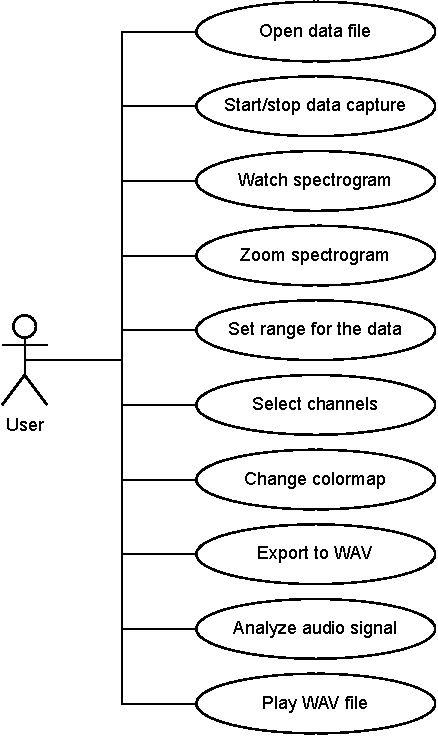
\includegraphics{pdf/usecase.drawio.pdf}
    \caption{Application usecases}
    \label{fig:usecase}
\end{figure}

\subsection{Application requirements}

From the use cases in Section \ref{lab:usecases} it is understandable that the application should have certain features. Apart from the given use cases, there are other important requirements:

\begin{itemize}
    \item Support for real-time data plotting - graph updates or animation; fetching the data online from the OptaSense Interrogator and displaying it in real-time
    \item Multiplatform - the application should run on any device and still support all features
    \item Data processing - subsampling data to save data throughput
    \item Plot editing and animation - changing plot properties
    \item Reading offline data - possibility to read local files or upload files into the application
    % \item 
\end{itemize}

% There is the option to create an application running on the operating system

\begin{figure}[h]
    \centering
    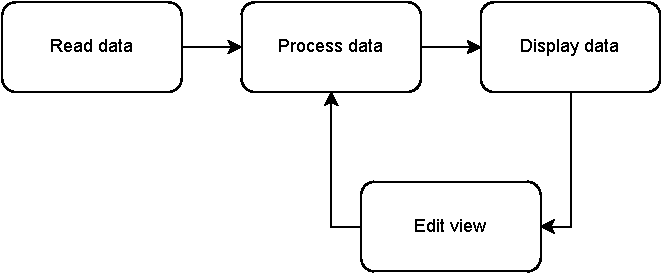
\includegraphics{pdf/simple_application.drawio.pdf}
    \caption{Data flow in the application - reading the data then processing the data and displaying it (optionally) edit the view}
    \label{fig:dataflow}
\end{figure}

It is necessary to choose the right programming tools to satisfy all features. The right way to find the right solution in programming is to \textit{divide and conquer}. This means finding all the pieces that will make the application. First, there must be an idea of what will happen with the data. Firstly, it has to be read, processed, and then displayed, the optional step is to edit the data or change the view; this data flow can be seen in Figure \ref{fig:dataflow}. 

% Multiplatform requirement removes many options - like creating a simple GUI application, as creating a multiplatform high-performance application is quite a feat and is beyond this project. So the result is making a web site and display  there is one solution either using 

From the data flow application, an overview can be made for a web application, as can be seen in Figure \ref{fig:app_overview}. The overview illustrates what parts the application will have. The back-end or server application will be responsible for reading HDF5 files and processing data. It will provide some form of interface or API for the client application to fetch\footnote{\url{https://developer.mozilla.org/en-US/docs/Web/API/Fetch\_API}} the data. On the client side, the client has to be able to create visualizations of the data and provide a user interface to change application properties.

\begin{figure}
    \centering
    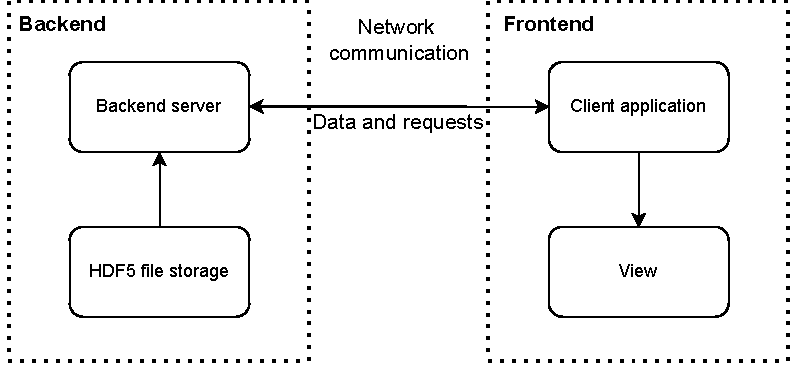
\includegraphics{pdf/appstack_general.drawio.pdf}
    \caption{Application overview. The server reads the data from the data storage and sends it to the client application, where it is shown to the user}
    \label{fig:app_overview}
\end{figure}

\section{Existing technology for data visualization}

This section focuses on data processing and visualization using existing software for visualizing scientific data. First is OptaSense OS6 software which is a purpose-made solution for OptaSense devices. Next is the h5web library, written in React, which creates a web page for visualizing the content of HDF5 files.

\subsection{OptaSense OS6}\label{sec:ossix}

The OptaSense company provides visualization software for their devices called OptaSense OS6\footnote{\url{https://www.optasense.com/technology/os/}}. It runs only on the Windows operating system. OS6 provides features for monitoring certain areas or land, for example, a compound or an industrial building. This product is tailor-made for OptaSense devices by the OptaSense company. This system has only one window for everything. The main view is the monitored area; the background picture is the aerial view of the whole monitored space, as can be seen in the picture \ref{fig:ossix}. The user can open the sidebar on the right side. The sidebar provides multiple different options:

\begin{itemize}
    \item \textbf{Spectrogram} - Raw data visualization.
    \item \textbf{Alerts} - When an action is detected along the wire, it is logged.
    \item \textbf{Notifications} -  Notifications about system state.
    \item \textbf{System status} - Overview of all OptaSense units and their state.
\end{itemize}

There is also a feature that takes raw data from interrogator units and processes them using machine learning. In this way, different actions are detected and categorized into different types of alerts, such as walking, driving cars, etc. In addition, the user can see the activities that were detected and triggered in the area overview with live monitoring and a timeline at the top of the screen. To easily look at different locations or start a new view, there is a feature \textit{type to search} that lets the user start a search by typing into the view. For example, the user starts writing ``water...'' as a waterfall, and the program will look for this feature and open the waterfall visualization window. OS6 saves all detected activities, which can be shown in the \textit{Historic timeline} window, which shows all alerts that occurred during a specified time range. The animations look very nice, although some of them look a bit choppy mostly when showing activities on top of the waterfall view. 

Anyway, it is proof that it is possible to create a real-time data visualization from the DAS system. It lacks one important step, which is the ability to be used not only on Windows machines and to be truly multiplatform.

\begin{figure}[]
    \centering
    \includegraphics[width=\linewidth]{obrazky/OSsix.png}
    \caption{OptaSense OS6 visualization software \cite{ytossix}}
    \label{fig:ossix}
\end{figure}

\subsection{h5web}

The \verb|h5web|\footnote{\url{https://h5web.panosc.eu/}} library is a set of components written in React\footnote{React is a JavaScript library used to create interactive user interface \url{https://reactjs.org/}}. H5web uses existing HDF5 libraries, such as h5wasm (reading HDF5 files in the browser) and h5grove (server for accessing HDF5 files). It displays the contents of HDF5 file, as well as shows different graphs according to the input from the user. From the presentation of the library by its developer it is safe to say that although it provides the necessary equipment for opening HDF5 files elegantly and provides advanced graphing techniques it lacks the ability to receive the data and display them in real-time. For this purpose, the library would need to add support by creating a new React component capable of such behavior, but it is possible.

\subsection{Backend}

The purpose of the backend part of the application is to read, process, and send the data to the client part of the application, as can be seen in Figure \ref{fig:app_overview}. Reading the HDF5 data is done as explained in Section \ref{sec:readhdf}.

\subsubsection{REST servers}

There is a wide range of REST server implementations; HDF Group provides documentation for its RESTful API\footnote{\url{https://support.hdfgroup.org/pubs/papers/RESTful\_HDF5.pdf}}. They have prepared a few RESTful server implementations for their data format. There are many more implementations of REST servers, such as the Python Simple HTTP server. Here is a list of some possible implementations \cite{hdfrest}:

\begin{itemize}
    \item \emph{h5serv} - REST-based service to access HDF5 data written in Python (HDF5 Group).
    \item \emph{HSDS} (Highly Scalable Data Service)\footnote{\url{https://github.com/HDFGroup/hsds}} - Python implementation of the REST-based service to access HDF5 data stores. Data can be stored in the POSIX file system or using object-based storage such as AWS S3. It can run in a Docker as a single machine or on a Kubernetes cluster.
    \item \emph{hdf-rest-api}\footnote{https://github.com/HDFGroup/hdf-rest-api} - is HDF5 REST API that provides CRUD support (create, read, update, and delete) for all HDF5 objects.
    \item \emph{h5grove} - Backend service written in Python providing access to HDF5 file content.
    \item \emph{http.server} - Python implementation of a simple HTTP server. However, this is better used only for testing purposes when accessing local files.
\end{itemize}

\subsubsection{WebSockets}

WebSockets (or WebSocket API) enable two-way communication over TCP. It was standardized by IEFT in RFC6455. WebSocket protocol is supported by all modern browsers. The communication starts with an HTTP-compatible handshake, so only one socket can be used to communicate with the server. There are also other header types available for different uses. The server responds with an HTTP Upgrade, the connection is established, and bidirectional communication can begin. Communication closes when either side decides to close the connection and starts closing the handshake. The other side responds with a \textit{Close frame} message and the connection is closed. The protocol is trying to be frame-based as is HTTP but also frame-based as little as possible, just to make sure that it can use the HTTP interface for communication; otherwise it tries to be as minimalist as possible. The authors of the WebSocket protocol wanted it to be low-level and as close to TCP as possible \cite{websock}. WebSockets have an implementation in the Python programming language called \verb|websockets|\footnote{https://pypi.org/project/websockets/}.

\begin{figure}[h]
    \centering
    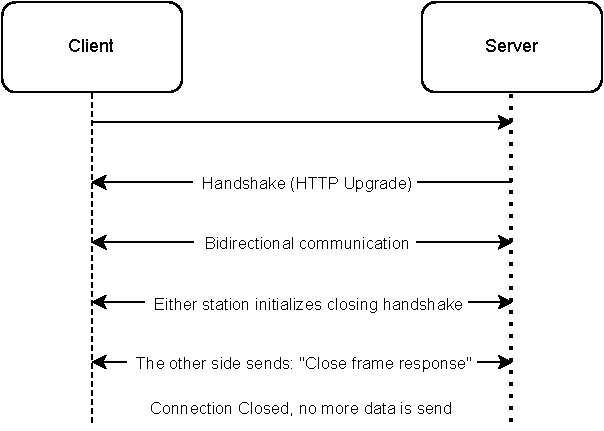
\includegraphics{pdf/websocket.drawio.pdf}
    \caption{WebSocket handshake, communication, and connection close diagram.}
    \label{fig:websocket}
\end{figure}

% \subsubsection{Processing data}\label{lab:processingdata}

% The data read from the file is in 

% %TODO







\subsection{Frontend}

% \subsubsection{WebGL}

% WebGL is a cross-platform web standard for 3D graphics API based on OpneGL, that is rendering into HTML \verb|<canvas>| element. It supports 
% https://github.com/bastibe/WebGL-Spectrogram


\subsubsection{Svelte}

Svelte is a component framework written in JavaScript, using a new approach to building web applications. Instead of looking for differences in virtual DOMs as React does, which is done in the browser and consumes quite a lot of resources, Svelte does everything at the compilation stage. The output of the compilation is a JavaScript file \verb|bundle.js|, which contains all the necessary code to run the web application or better said, it manipulates the DOM directly. The result is a fast and reactive web page, it also saves resources, and the code can be run on small devices like handheld devices. Web development is also very enjoyable because compilation does not take long and the result of changes can be visible immediately. Svelte also integrates CSS stylesheets into the components. The structure of a Svelte component consists of three parts - JavaScript code tag \verb|<script>| a style tag \verb|<style>| and other HTML elements. 

Svelte is capable of client-side rendering and server-side rendering, but it does not provide more advanced features like page routing. For this purpose, the Svelte team created SvelteKit, which is a~framework for building web applications and allows page routing. Routing is folder-based - the developer creates routing by creating a folder and file structure.

\begin{verbatim}
src/routes/about/+page.svelte <=> /about
src/routes/about.svelte <=> /about
\end{verbatim}

Svelte has been changing and has become a Vite \footnote{\url{https://vitejs.dev}} plugin. Vite provides fast development experience by running a development server, in the case of Svelte - Hot Module Replacement (HMR)\footnote{\url{https://vitejs.dev/guide/features.html\#hot-module-replacement}}. This way, every change made during development can be immediately seen in the browser without reloading the page, which makes development much faster and more enjoyable. It is necessary to say that Svelte is still in development and although it is now at version 3 it is possible that it will change in the future. 

When fetching the data from the server, it is good practice to move this functionality to a Svelte Store. The Svelte store is a separate JavaScript file that can be accessed from multiple components. From a programming point of view, a store is an object with a \verb|subscribe()| function. An example of a WebSocket implementation in Svelte can be the Svelte component library \textit{svelte-websocket-store}\footnote{\url{https://github.com/arlac77/svelte-websocket-store}}.

\subsection{Real-time capabilities}

The data bandwidth (the amount of data necessary to be sent from the server side to the client side) of the application is the biggest factor. The OptaSense Interrogator can produce quite a lot of data, but if it is saved in an HDF5 file, it is quite small. As discussed in Section \ref{sec:readhdf}, a \qty{10}{\second} file produces around \qty{52}{MB} of data. When this data is transformed into text form, it has only \qty{420}{MB} and when transformed into JSON, it has \qty{946}{MB} as the data are read at \ac{SPS} \qty{10}{kSPS}\footnote{\ac{SPS}}. Data will be displayed on a display with standard resolution and cannot display \qty{10000}{SPS} on a small part of the display. Data processing is necessary for this purpose. 

% \subsubsection{Data processing}

% Data processing can be done on the server side or in the browser. As the browser will be busy redrawing waterfall visualization it is better to do data preprocessing on the server side. Server-side preprocessing will also save bandwidth as the data will be significantly filtered. 

% Sending data in the form of REST requests and responses can be possible but it is really useful only when sending a small HDF5 file as a whole not as a stream of data and although h5grove backend provides the ability to read sections of the data set for  The respective bandwidth would be \qty{}{}



% %TODO


 % The JSON file is quite large - the original HDF5 file is only \qty{52,7}{MB} and the JSON file is \qty{946,6}{MB}. The dump text file is half the size and provides the same information, but the datasets are harder to understand, but the whole file is only half the size of the JSON file at ``only'' \qty{420}{MB}. The JSON format is much easier to read. The structure of the file is divided into three parts:

\subsection{Software design for DAS data visualization}

As we discussed in Section \ref{sec:ossix}, it is possible to create such software to display the data in real time. The application was a native Windows application, and the requirement for this application was to be able to run on multiple platforms. The chosen platform is the Python backend, opening files, processing the data, and sending the data into the client application using Svelte. The backend will process the data as explained in \ref{lab:processingdata}. The waterfall graph will be an HTML Canvas element that displays the data in real-time, redrawing itself as the data arrive at the browser. For ease of displaying the data in Canvas, D3js will be used. D3 will, for example, apply a color map to the correct scale according to the data. The user interface written in Svelte will also have inputs to change the properties of the visualization so that the user can select specific channels from the data, choose subsampling effect properties, cutting the frequency range. The ability to export the data to a WAV file will also be implemented the same way as done in Section \ref{lab:hdftowav}.

\begin{figure}
    \centering
    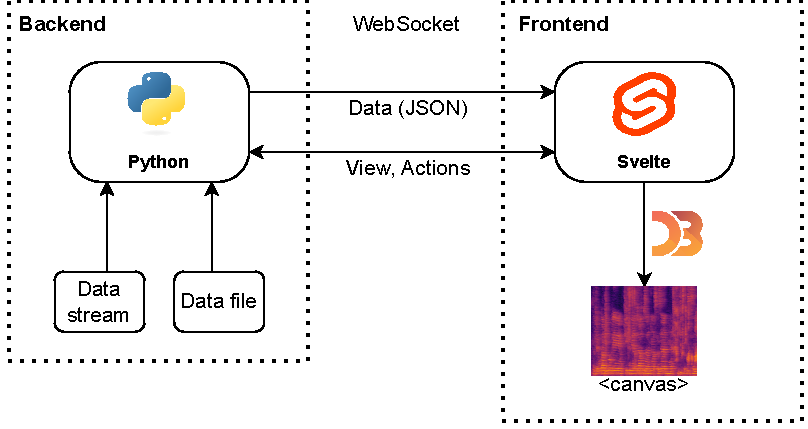
\includegraphics{obrazky/appstack.drawio.pdf}
    \caption{Application overview}
    \label{fig:app_overview}
\end{figure}

\subsection{Prototype}

This work aims to design an application to visualize HDF5 data acquired from the OptaSense Interrogator. For this purpose, Svelte was used mainly for its high performance, thanks to efficient code created at compilation. This is a prototype, so it is not a working application. It is only to show how this application will look in the end. The final version of the application will also use Svelte. The prototype uses Flowbite components\footnote{\url{https://flowbite-svelte.com/}} as they make it easy to create stylized web pages. The web page is divided into Svelte components. The main component is the waterfall graph on the left side of the screen and the control panel on the right side. Layout is done with svelte-layouts\footnote{\url{https://www.npmjs.com/package/svelte-layouts}} package. 

Uploading files into the browser using REST API was also tested. Python's \verb|http.server| was used as the backend. When fetching files into a browser from local storage using HTTP, it is necessary to allow Cross-Origin Resource Sharing (CORS) because browsers restrict this feature for security reasons. Some resources like CSS, Web Fonts, and WebGL textures have enabled CORS. For sending HDF5 files to the browser, a special HTTP header has to be added on the server side. Without this feature, the browser would throw an error into the JavaScript console.

\begin{figure}
    \centering
    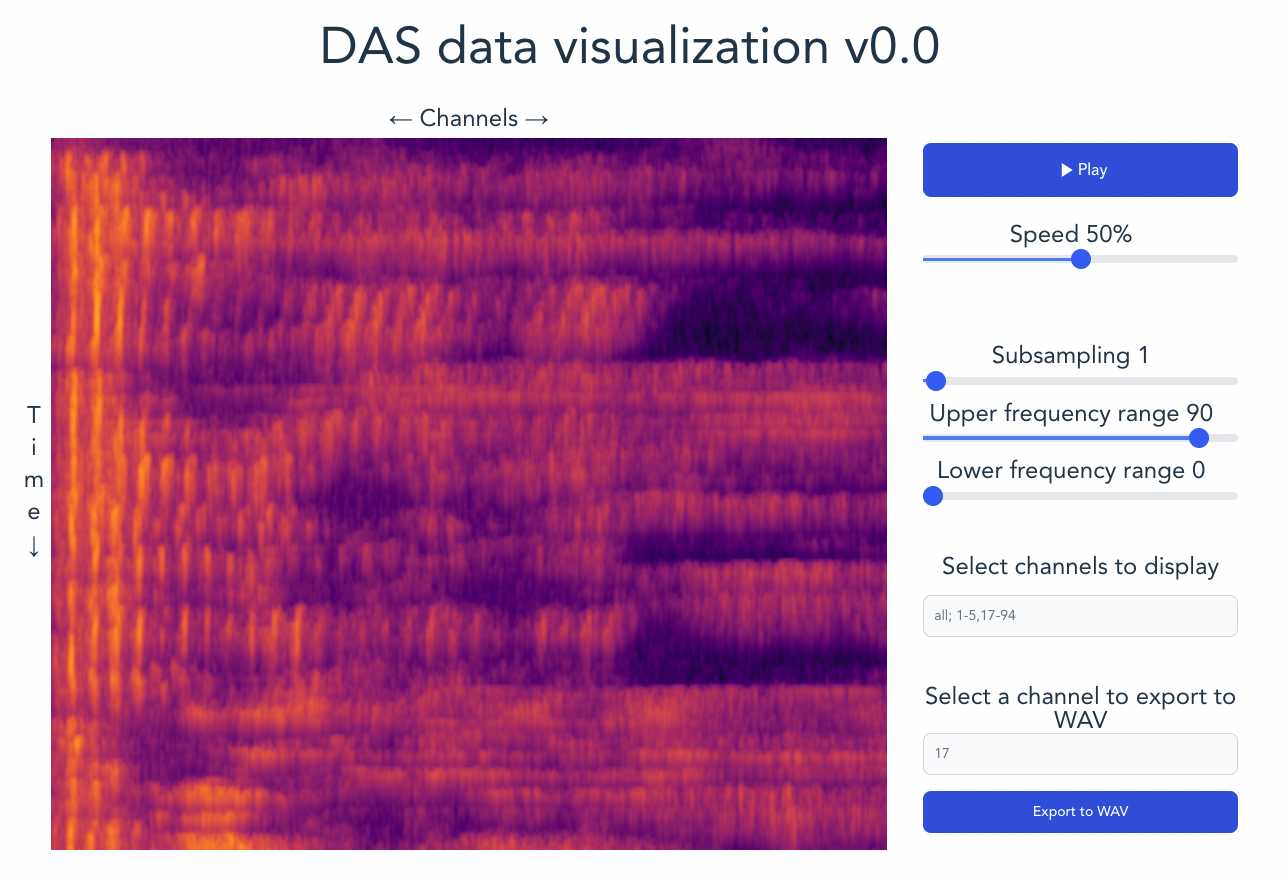
\includegraphics[width=\linewidth]{obrazky/svelte_prototype.png}
    \caption{Prototype of DAS visualization application}
    \label{fig:prototypesvelte}
\end{figure}


%%% Vložení souboru 'text/vysledky' s popisem vysledků práce
% (rozdělte na více souborů či kapitol, pokud je vhodné)
% \chapter{Výsledky studentské práce}

Praktická část a výsledky studentské práce vhodně rozdělené do částí.

\section{Programové řešení}
Lorem ipsum dolor sit amet, consectetuer adipiscing elit. Nulla pulvinar eleifend sem. Integer in sapien. Etiam sapien elit, consequat eget, tristique non, venenatis quis, ante. In laoreet, magna id viverra tincidunt, sem odio bibendum justo, vel imperdiet sapien wisi sed libero. Phasellus enim erat, vestibulum vel, aliquam a, posuere eu, velit. Aliquam erat volutpat. Nullam faucibus mi quis velit \cite{sr02/2009}.

\section{Výsledky měření}
Fusce tellus odio, dapibus id fermentum quis, suscipit id erat. Fusce tellus. Morbi scelerisque luctus velit. In laoreet, magna id viverra tincidunt, sem odio bibendum justo, vel imperdiet sapien wisi sed libero. Quisque porta. Fusce suscipit libero eget elit. Nulla non lectus sed nisl molestie malesuada. Phasellus faucibus molestie nisl. Integer vulputate sem a nibh rutrum consequat. Proin mattis lacinia justo. Phasellus et lorem id felis nonummy placerat. Etiam ligula pede, sagittis quis, interdum ultricies, scelerisque eu. Cras elementum. Aenean placerat. Donec ipsum massa, ullamcorper in, auctor et, scelerisque sed, est. Aliquam ante. Integer imperdiet lectus quis justo. Vivamus ac leo pretium faucibus. Nullam faucibus mi quis velit.

\subsection{Etiam quis quam}
Neque porro quisquam est, qui dolorem ipsum quia dolor sit amet, consectetur, adipisci velit, sed quia non numquam eius modi tempora incidunt ut labore et dolore magnam aliquam quaerat voluptatem. Aliquam erat volutpat. Lorem ipsum dolor sit amet, consectetuer adipiscing elit \cite{sr02/2009,pravidla}. Nunc auctor. Neque porro quisquam est, qui dolorem ipsum quia dolor sit amet, consectetur, adipisci velit, sed quia non numquam eius modi tempora incidunt ut labore et dolore magnam aliquam quaerat voluptatem. Maecenas lorem. Maecenas libero. In laoreet, magna id viverra tincidunt, sem odio bibendum justo, vel imperdiet sapien wisi sed libero. Nullam rhoncus aliquam metus.

\subsubsection{Integer rutrum orci vestibulum}
Integer rutrum, orci vestibulum ullamcorper ultricies, lacus quam ultricies odio, vitae placerat pede sem sit amet enim. Ut enim ad minim veniam, quis nostrud exercitation ullamco laboris nisi ut aliquip ex ea commodo consequat. Fusce tellus odio, dapibus id fermentum quis, suscipit id erat. Nullam eget nisl. Nunc auctor. Etiam dui sem, fermentum vitae, sagittis id, malesuada in, quam. Fusce dui leo, imperdiet in, aliquam sit amet, feugiat eu, orci. Curabitur vitae diam non enim vestibulum interdum. Aliquam erat volutpat. Pellentesque sapien. Phasellus enim erat, vestibulum vel, aliquam a, posuere eu, velit.

\subsubsection{Eger rutrum orci westibulum}
Fusce dui leo, imperdiet in, aliquam sit amet, feugiat eu, orci. Maecenas aliquet accumsan leo. Aliquam ornare wisi eu metus. Cum sociis natoque penatibus et magnis dis parturient montes, nascetur ridiculus mus. Aliquam erat volutpat. Donec iaculis gravida nulla. Sed elit dui, pellentesque a, faucibus vel, interdum nec, diam. Temporibus autem quibusdam et aut officiis debitis aut rerum necessitatibus saepe eveniet ut et voluptates repudiandae sint et molestiae non recusandae. Nulla non arcu lacinia neque faucibus fringilla. Phasellus enim erat, vestibulum vel, aliquam a, posuere eu, velit. Praesent vitae arcu tempor neque lacinia pretium
\cite{Walter1999,Svacina1999IEEE,RajmicSysel2002}.

Aliquam erat volutpat. Quisque porta. Integer imperdiet lectus quis justo. Nullam justo enim, consectetuer nec, ullamcorper ac, vestibulum in, elit. Nullam faucibus mi quis velit. Fusce tellus. Fusce consectetuer risus a nunc. Cras pede libero, dapibus nec, pretium sit amet, tempor quis. Morbi imperdiet, mauris ac auctor dictum, nisl ligula egestas nulla, et sollicitudin sem purus in lacus
\cite{CSN_ISO_690-2011,CSN_ISO_7144-1997,CSN_ISO_31-11}.
Mauris elementum mauris vitae tortor. Neque porro quisquam est, qui dolorem ipsum quia dolor sit amet, consectetur, adipisci velit, sed quia non numquam eius modi tempora incidunt ut labore et dolore magnam aliquam quaerat voluptatem. Quisque porta. Integer vulputate sem a nibh rutrum consequat. Nulla pulvinar eleifend sem. Praesent id justo in neque elementum ultrices \cite{BiernatovaSkupa2011:CSNISO690komentar}.

Fusce suscipit libero eget elit. Integer vulputate sem a nibh rutrum consequat. Aliquam erat volutpat. Etiam neque. Nulla turpis magna, cursus sit amet, suscipit a, interdum id, felis. Nullam rhoncus aliquam metus. Etiam dui sem, fermentum vitae, sagittis id, malesuada in, quam. Nunc auctor. Nunc dapibus tortor vel mi dapibus sollicitudin. Praesent in mauris eu tortor porttitor accumsan. Nulla non arcu lacinia neque faucibus fringilla. Nullam lectus justo, vulputate eget mollis sed, tempor sed magna. Maecenas lorem. Aenean placerat. Donec vitae arcu. Maecenas lorem. Donec iaculis gravida nulla. Nulla non lectus sed nisl molestie malesuada.

Duis pulvinar. Nulla est. Duis condimentum augue id magna semper rutrum. Integer pellentesque quam vel velit. Aliquam ante. Nulla quis diam. Proin mattis lacinia justo. Aenean fermentum risus id tortor. Nunc auctor. Nullam justo enim, consectetuer nec, ullamcorper ac, vestibulum in, elit. In dapibus augue non sapien. Etiam bibendum elit eget erat. In sem justo, commodo ut, suscipit at, pharetra vitae, orci. Maecenas libero.

Nulla non lectus sed nisl molestie malesuada. Donec vitae arcu. Aenean fermentum risus id tortor. Praesent in mauris eu tortor porttitor accumsan. Nulla pulvinar eleifend sem. Duis viverra diam non justo. Integer imperdiet lectus quis justo. Pellentesque habitant morbi tristique senectus et netus et malesuada fames ac turpis egestas. In rutrum. Excepteur sint occaecat cupidatat non proident, sunt in culpa qui officia deserunt mollit anim id est laborum. Nulla non lectus sed nisl molestie malesuada. Aliquam erat volutpat. Mauris tincidunt sem sed arcu. Duis bibendum, lectus ut viverra rhoncus, dolor nunc faucibus libero, eget facilisis enim ipsum id lacus. Fusce tellus odio, dapibus id fermentum quis, suscipit id erat. In enim a arcu imperdiet malesuada. Nulla non lectus sed nisl molestie malesuada. Proin mattis lacinia justo.

Aliquam in lorem sit amet leo accumsan lacinia. Cum sociis natoque penatibus et magnis dis parturient montes, nascetur ridiculus mus. Duis sapien nunc, commodo et, interdum suscipit, sollicitudin et, dolor. Suspendisse sagittis ultrices augue. Nullam lectus justo, vulputate eget mollis sed, tempor sed magna. In convallis. Praesent id justo in neque elementum ultrices. Neque porro quisquam est, qui dolorem ipsum quia dolor sit amet, consectetur, adipisci velit, sed quia non numquam eius modi tempora incidunt ut labore et dolore magnam aliquam quaerat voluptatem.

Pellentesque pretium lectus id turpis. Nemo enim ipsam voluptatem quia voluptas sit aspernatur aut odit aut fugit, sed quia consequuntur magni dolores eos qui ratione voluptatem sequi nesciunt. Curabitur ligula sapien, pulvinar a vestibulum quis, facilisis vel sapien. Praesent dapibus. Sed elit dui, pellentesque a, faucibus vel, interdum nec, diam. Duis viverra diam non justo. Duis ante orci, molestie vitae vehicula venenatis, tincidunt ac pede. Phasellus rhoncus. Maecenas fermentum, sem in pharetra pellentesque, velit turpis volutpat ante, in pharetra metus odio a lectus. Proin pede metus, vulputate nec, fermentum fringilla, vehicula vitae, justo. Fusce aliquam vestibulum ipsum. Nullam at arcu a est sollicitudin euismod.

%Aliquam ante. Phasellus faucibus molestie nisl. Etiam ligula pede, sagittis quis, interdum ultricies, scelerisque eu. Morbi leo mi, nonummy eget tristique non, rhoncus non leo. Cum sociis natoque penatibus et magnis dis parturient montes, nascetur ridiculus mus. Morbi scelerisque luctus velit. Curabitur bibendum justo non orci. Donec quis nibh at felis congue commodo. Nullam faucibus mi quis velit. Aenean id metus id velit ullamcorper pulvinar. Pellentesque sapien. Fusce nibh. Vestibulum fermentum tortor id mi. Nullam eget nisl. Praesent vitae arcu tempor neque lacinia pretium. Proin in tellus sit amet nibh dignissim sagittis. Donec quis nibh at felis congue commodo.
%
%Nam quis nulla. Proin in tellus sit amet nibh dignissim sagittis. Nullam dapibus fermentum ipsum. Curabitur ligula sapien, pulvinar a vestibulum quis, facilisis vel sapien. Nam libero tempore, cum soluta nobis est eligendi optio cumque nihil impedit quo minus id quod maxime placeat facere possimus, omnis voluptas assumenda est, omnis dolor repellendus. Vivamus ac leo pretium faucibus. Nunc tincidunt ante vitae massa. Maecenas sollicitudin. Ut tempus purus at lorem. Nullam lectus justo, vulputate eget mollis sed, tempor sed magna. Fusce consectetuer risus a nunc. Etiam quis quam.
%
%Donec quis nibh at felis congue commodo. Sed vel lectus. Donec odio tempus molestie, porttitor ut, iaculis quis, sem. Nullam feugiat, turpis at pulvinar vulputate, erat libero tristique tellus, nec bibendum odio risus sit amet ante. Sed elit dui, pellentesque a, faucibus vel, interdum nec, diam. Cras elementum. Sed vel lectus. Donec odio tempus molestie, porttitor ut, iaculis quis, sem. Etiam neque. Integer tempor. Vivamus porttitor turpis ac leo. Nulla non arcu lacinia neque faucibus fringilla.
%
%Etiam posuere lacus quis dolor. Nemo enim ipsam voluptatem quia voluptas sit aspernatur aut odit aut fugit, sed quia consequuntur magni dolores eos qui ratione voluptatem sequi nesciunt. Nullam faucibus mi quis velit. Cum sociis natoque penatibus et magnis dis parturient montes, nascetur ridiculus mus. Phasellus faucibus molestie nisl. Maecenas ipsum velit, consectetuer eu lobortis ut, dictum at dui. Maecenas aliquet accumsan leo. Pellentesque ipsum. Donec vitae arcu. Suspendisse nisl. Morbi imperdiet, mauris ac auctor dictum, nisl ligula egestas nulla, et sollicitudin sem purus in lacus. Pellentesque ipsum. Ut enim ad minima veniam, quis nostrum exercitationem ullam corporis suscipit laboriosam, nisi ut aliquid ex ea commodi consequatur? Nam libero tempore, cum soluta nobis est eligendi optio cumque nihil impedit quo minus id quod maxime placeat facere possimus, omnis voluptas assumenda est, omnis dolor repellendus.


%%% Vložení souboru 'text/zaver' se závěrem
\chapter*{Conclusion}
\phantomsection
\addcontentsline{toc}{chapter}{Conclusion}

The main goal of this work was to study the~DAS system and its output files in~the~HDF5 file format. As for the~implementation part, the~goal was to create a~multi-platform application capable of displaying the~data from the~DAS interrogator, processing it, and displaying it in a~suitable form. The visualization should be able to play and pause the~animation of the~flowing data, also with the~ability to convert the~data into an audio file.  

In the~theoretical part, the~principles of optical reflectometry were explained, as well as different types of light scattering - Mie scattering, Rayleigh scattering, Raman scattering, and Brillouin scattering. the~inner workings of the~DAS system and methods like \ac{generalotdr} and \ac{otdr} were also studied. The output file format HDF5 was carefully examined with objects such as Datasets, Groups, Attributes, and Links. The output file structure of the~DAS system OptaSense ODH-F was shown in a~readable form. The existing technology was studied with available software for the~front-end and server side. Real-time capabilities were also discussed with the~data bandwidth requirements. A~prototype was created and written in~Svelte to showcase the~application's design with a~waterfall graph and HTML elements to set properties for display. 

In the~design section, we discuss software requirements and the~basic back-end technologies used later in the~implementation section, such as WebSockets and reading HDF5 files. The front-end technologies for data visualization based on Canvas and SVG graphics were discussed. The basics of the~Svelte framework were introduced.

A web application was created with a~server written in Python and a~client using the~Svelte framework. The back end can read and process the~data in HDF5 file format. The back-end communicates with the~client side using WebSockets. A~simple message system was created for this purpose. The client allows the~user to choose the~file and the~dataset, as well as properties like speed choosing a~colormap and channels to display. The visualization can be started, stopped, and replayed. There is also a~feature to download the~image currently on display.

% In the~last section the~software design of a~real-time application for the~DAS system was discussed. 


% The work can be used as a~resource for creating an application for data visualization in the~browser. The next step is to create fully functional web application - with its server-side written in Python sending data using WebSockets to the~front-end client application written in Svelte.

The application in this state is a~one-page website; the~next step would be to incorporate it into the~SvelteKit framework, allowing page routing. This should be pretty straightforward. Future work can include further improving the~visualization, including zooming and data selection features, either by creating custom \texttt{<canvas>} rendering, SVG rendering with D3js, or using existing libraries such as Plotly. It~might be useful to have multiple algorithms to choose from when processing the~raw DAS data. Although we tried a~few methods for data processing, we have chosen one, and there is no selection possible at this stage.





% \section{}

% The semestral part of the~thesis studies DAS principles

% and the output format of the deployed system, 

% \section{Implementation}

% followed by an implementation of conversion from data to audio signal (in WAV format). 

% \subsection{Real-time possibilities}

% This part also investigates the possibilities of real-time data analysis



% Práce je zaměřena na analýzu dat z optického distribuovaného akustického senzorického (DAS) systému ve formátu HDF5. V semestrální práci student prostuduje princip DAS systém a~jeho výstupy (HDF5 archivy) s detailním popisem formátu HDF5. Následně navrhne program pro převod dat do akustické podoby (WAV) a~popíše možnosti realizace programu v reálném čase. V diplomové práci bude navrženo grafické rozhraní zobrazující data v čase s možnostmi úprav os grafu. Výsledek bude otestován s reálným DAS systémem a~fakultním optickým senzorickým polygonem.




% Info o systeme co pouzivaju v tyme
% 	HW info
% 	outputformat - popisat atributy, kanaly, a~celkovo ako to uklada to toho hdf5ky




% Obsah:
% ako to funguje
% existujuci HW


%%% Vložení souboru 'text/literatura' se seznamem zdrojů
% Pro sazbu seznamu literatury použijte jednu z následujících možností

%%%%%%%%%%%%%%%%%%%%%%%%%%%%%%%%%%%%%%%%%%%%%%%%%%%%%%%%%%%%%%%%%%%%%%%%%
%1) Seznam citací definovaný přímo pomocí prostředí literatura / thebibliography

\begin{thebibliography}{99}

\bibitem{WangYu2017RDVM}

WANG, Yu, Baoquan JIN, Yuncai WANG, Dong WANG, Xin LIU, Qing BAI: \emph{Real-Time Distributed Vibration Monitoring System Using $\Phi$-OTDR}. IEEE sensors journal [online]. PISCATAWAY: IEEE, 2017, 17(5), 1333-1341 [cit. 2022-11-22]. ISSN 1530-437X. Accessible at: doi:10.1109/JSEN.2016.2642221

\bibitem{dasKislov}
KISLOV, K. V. a V. V. GRAVIROV: \emph{Distributed Acoustic Sensing: A New Tool or a New Paradigm. Seismic instruments} [online]. Moscow: Pleiades Publishing, 2022, 58(5), 485-508 [cit. 2022-11-22]. ISSN 0747-9239. Accessible at: doi:10.3103/S0747923922050085

\bibitem{dasseismic}
PARKER, Tom, SHATALIN, Sergey, FARHADIROUSAN Mahmoud: \emph{Distributed Acoustic Sensing – a new tool for seismic applications}. Earthdoc [online]. [cit. 2022-11-22]. Accessible at \(<\)\url{https://doi.org/10.3997/1365-2397.2013034}\(>\)

\bibitem{gabai}
GABAI, Haniel, and AVISHAY Eyal: \emph{On the sensitivity of distributed acoustic sensing.} Optics letters vol. 41,24 (2016): 5648-5651. [online]. [cit. 2022-11-22] doi:10.1364/OL.41.005648

\bibitem{wangprogress}
WANG Z, LU B, YE Q, CAI H.: \emph{Recent Progress in Distributed Fiber Acoustic Sensing with $\Phi$-OTDR}. Sensors (Basel). 2020 Nov 18;20(22):6594. doi: 10.3390/s20226594. PMID: 33218051; PMCID: PMC7698859.

\bibitem{kislov_das_newparadigm}
KISLOV, K. V. a V. V. GRAVIROV.: \emph{Distributed Acoustic Sensing: A New Tool or a New Paradigm. Seismic instruments} [online]. Moscow: Pleiades Publishing, 2022, 58(5), 485-508 [cit. 2022-11-25]. ISSN 0747-9239. Accessible at: doi:10.3103/S0747923922050085

\bibitem{hdf5doc}
\emph{The HDF5 Data Model and File Structure} HDF Group [cit. 2022-12-08]. Accessible at \(<\)\url{https://docs.hdfgroup.org/hdf5/develop/_h5_d_m__u_g.html}\(>\).

\bibitem{hdfrest}
HEBER G.: \emph{RESTful HDF5} The HDF Group [cit. 2022-12-08].
\(<\)\url{https://support.hdfgroup.org/pubs/papers/RESTful_HDF5.pdf}\(>\).

\bibitem{seismic}
HORNMAN, J.C.: \emph{Field trial of seismic recording using distributed acoustic sensing with broadside sensitive fibre-optic cables.} Geophysical Prospecting [online]. 2017, 65(1), 35-46 [cit. 2022-12-06]. ISSN 0016-8025. Accessible at: doi:10.1111/1365-2478.12358

\bibitem{progress}
BAO, Xiaoyi a Liang CHEN.: \emph{Recent Progress in Distributed Fiber Optic Sensors}. Sensors (Basel, Switzerland) [online]. BASEL: Mdpi, 2012, 12(7), 8601-8639 [cit. 2022-12-08]. ISSN 1424-8220. Accessible at: doi:10.3390/s120708601

\bibitem{dasrayleigh}
PALMIERI, Luca; SCHENATO, Luca. Distributed optical fiber sensing based on Rayleigh scattering. The Open Optics Journal, 2013, 7.1.

\bibitem{ytossix}
OptaSense OS6 Visualization Software Demo. YouTube, uploaded by OptaSense, 22 June 2021, \(<\)\url{https://www.youtube.com/watch?v=6-hj1ySERIA}\(>\).

\bibitem{websock}
Melnikov, A., Fette, I.: \emph{The WebSocket Protocol}. RFC Editor. [online] [cit. 2022-08-12]. Accessible at: \(<\)\url{https://doi.org/10.17487/RFC6455}\(>\).

\bibitem{cors} 
\emph{Cross-Origin Resource Sharing (CORS)} mozilla.org [cit. 2022-12-08]. Accessible at \(<\)\url{https://developer.mozilla.org/en-US/docs/Web/HTTP/CORS}\(>\).


% @misc{rfc6455,
%     series =    {Request for Comments},
%     number =    6455,
%     howpublished =  {RFC 6455},
%     publisher = {RFC Editor},
%     doi =       {10.17487/RFC6455},
%     url =       {https://www.rfc-editor.org/info/rfc6455},
%         author =    {Alexey Melnikov and Ian Fette},
%     title =     {{The WebSocket Protocol}},
%     pagetotal = 71,
%     year =      2011,
%     month =     dec,
%     abstract =  {The WebSocket Protocol enables two-way communication between a client running untrusted code in a controlled environment to a remote host that has opted-in to communications from that code. The security model used for this is the origin-based security model commonly used by web browsers. The protocol consists of an opening handshake followed by basic message framing, layered over TCP. The goal of this technology is to provide a mechanism for browser-based applications that need two-way communication with servers that does not rely on opening multiple HTTP connections (e.g., using XMLHttpRequest or \textless{}iframe\textgreater{}s and long polling). {[}STANDARDS-TRACK{]}},
% }





% \bibitem{sr02/2009}
% 		VUT v~Brně:
%     \emph{Úprava, odevzdávání a zveřejňování vysokoškolských kva\-li\-fi\-kač\-ních prací na VUT v~Brně}\/ [online].
% 		Směrnice rektora č.\,2/2009.
% 		Brno: 2009, po\-sled\-ní aktualizace 24.\,3.\,2009 [cit.\,23.\,10.\,2015].
%     Dostupné z~URL:\\
%     <\url{https://www.vutbr.cz/uredni-deska/vnitrni-predpisy-a-dokumenty/smernice-rektora-f34920/}>.

% \bibitem{CSN_ISO_690-2011}
%     \emph{ČSN ISO 690 (01 0197) Informace a dokumentace -- Pravidla pro bibliografické odkazy a citace informačních zdrojů.}
%     40 stran. Praha: Český normalizační institut, 2011.

% \bibitem{CSN_ISO_7144-1997}
%     \emph{ČSN ISO 7144 (010161) Dokumentace -- Formální úprava disertací a podobných dokumentů.}
%     24 stran. Praha: Český normalizační institut, 1997.

% \bibitem{CSN_ISO_31-11}
%     \emph{ČSN ISO 31-11 Veličiny a jednotky -- část 11: Matematické znaky a značky používané ve fyzikálních vědách a v~technice.}
%     Praha: Český normalizační institut, 1999.

% \bibitem{BiernatovaSkupa2011:CSNISO690komentar}
%     BIERNÁTOVÁ, O., SKŮPA, J.:
%     \emph{Bibliografické odkazy a citace dokumentů dle ČSN ISO 690 (01 0197) platné od 1.\,dubna 2011}\/ [online].
%     2011, poslední aktualizace 2.\,9.\,2011 [cit. 19.\,10.\,2011].
%     Dostupné z~URL:
%     \(<\)\url{http://www.citace.com/CSN-ISO-690.pdf}\(>\)
%    \(<\)\href{http://www.boldis.cz/citace/citace.html}{http://www.boldis.cz/citace/citace.html}\(>\).

% \bibitem{pravidla}
%     \emph{Pravidla českého pravopisu}.
%     Zpracoval kolektiv autorů. 1.\ vydání.
%     Olomouc: FIN PUB\-LISH\-ING, 1998. 575 s. ISBN 80-86002-40-3.

% \bibitem{Walter1999}
% 	WALTER, G.\,G.; SHEN, X.
% 	\emph{Wavelets and Other Orthogonal Systems}.
% 	2. vyd. Boca Raton: Chapman\,\&\,Hall/CRC, 2000. 392~s. ISBN 1-58488-227-1

% \bibitem{Svacina1999IEEE}
% 	SVAČINA, J.
% 	Dispersion Characteristics of Multilayered Slotlines -- a Simple Approach.
% 	\emph{IEEE Transactions on Microwave Theory and Techniques},
% 	1999, vol.\,47, no.\,9, s.\,1826--1829. ISSN 0018-9480.

% \bibitem{RajmicSysel2002}
%     RAJMIC, P.; SYSEL, P.
%     Wavelet Spectrum Thresholding Rules.
%     In \emph{Proceedings of the International Conference Research in Telecommunication Technology},
%     Žilina: Žilina University, 2002. s.\,60--63. ISBN 80-7100-991-1.

\end{thebibliography}


%%%%%%%%%%%%%%%%%%%%%%%%%%%%%%%%%%%%%%%%%%%%%%%%%%%%%%%%%%%%%%%%%%%%%%%%%
%%2) Seznam citací pomocí BibTeXu
%% Při použití je nutné v TeXnicCenter ve výstupním profilu aktivovat spouštění BibTeXu po překladu.
%% Definice stylu seznamu
%\bibliographystyle{unsrturl}
%% Pro českou sazbu lze použít styl czechiso.bst ze stránek
%% http://www.fit.vutbr.cz/~martinek/latex/czechiso.tar.gz
%%\bibliographystyle{czechiso}
%% Vložení souboru se seznamem citací
%\bibliography{text/literatura}
%
%% Následující příkaz je pouze pro ukázku sazby literatury při použití BibTeXu.
%% Způsobí citaci všech zdrojů v souboru literatura.bib, i když nejsou citovány v textu.
%\nocite{*}

%%% Vložení souboru 'text/zkratky' se seznam použitých symbolů, veličin a zkratek
\cleardoublepage
\chapter*{\listofabbrevname}
\phantomsection
\addcontentsline{toc}{chapter}{\listofabbrevname}

\begin{acronym}[KolikMista]
        \acro{adm}
            [ADM]
            {Abstract Data Model}
        \acro{otdr}
            [$\Phi$-OTDR]
            {Phase-Sensitive Optical Time Domain Reflectometry}
        \acro{das}
            [DAS]
            {Distributed Acoustic Sensing}

        \acro{dss}
            [DSS]
            {Distributed Strain Sensing}

        \acro{dts}
            [DTS]
            {Distributed Temperature Sensing}
        \acro{dvs}
            [DVS]
            {Distributed Vibration Sensing}
        % \acro{}
        %     []
        %     {Distributed  Sensing}
        % \acro{}
        %     []
        %     {Distributed  Sensing}
   
        \acro{generalotdr}
            [OTDR]
            {Optic Time Domain Reflectometry}
        \acro{fft}
            [FFT]
            {Fast Fourier Transformation}
	   \acro{hdf}
            [HDF5]
            {Hierarchical Data Format v5}
        \acro{ofdr}
            [OFDR]
            {Optic Frequency Domain Reflectometry}
        \acro{sps}
            [SPS]
            {samples per second}

        \acro{svg}
            [SVG]
            {Scalable Vector Graphics}
        \acro{dthree}[D3.js]{Data-Driven Documents}
        \acro{dom}{DOM}{Document Object Model}
											% rozvinutí zkratky
	% \acro{zkTemp}		% název
	% 	[Šířka levého sloupce Seznamu symbolů a zkratek]								% zkratka
	% 	{je určena šířkou parametru prostředí \texttt{acronym} (viz řádek~1 výpisu zdrojáku na~str.\,\pageref{lst:zkratky})}
	% 										% rozvinutí zkratky

	% \acro{zkDummy}
	% 	[KolikMista]
	% 	{pouze ukázka vyhrazeného místa}

	% \acro{DSP}		% název/zkratka
	% 	{číslicové zpracování signálů -- Digital Signal Processing}
	% 										% rozvinutí zkratky
	% %%% bsymfvz
	% \acro{symfvz}						% název
	% 	[\ensuremath{f_\textind{vz}}] % symbol
	% 	{vzorkovací kmitočet}					% popis
	% %%% esymfvz

\end{acronym}


%%% Začátek příloh
\appendix

%%% Vysázení seznamu příloh
% (vynechejte, pokud máte dvě nebo méně příloh)
\listofappendices

%%% Vložení souboru 'text/prilohy' s přílohami
% Obvykle je přítomen alespoň popis co najdeme na přiloženém médiu
\chapter{Installing dependencies}\label{atach:dependencies}

Using a virtual environment is suggested and installing all dependencies in the environment.

\begin{verbatim}
    python3 -m venv env
    source env/bin/activate
    pip3 install -r requirements
\end{verbatim}

\section{Optasense visualizer application usage}\label{usage}

To run the application it is necessary to have an environment set up and all dependencies installed.
\textit{} \newline
Run the server part of the application:
\begin{verbatim}
    python3 app.py
\end{verbatim}

\textit{} \newline
The application usage:

\begin{verbatim}
usage: app.py [-h] [--port PORT]

DAS file visualization software. Server application.

options:
  -h, --help   show this help message and exit
  --port PORT  Port number for websocket.
\end{verbatim}


\section{Svelte}\label{attach:svelte}
\textit{} \newline
To create a Svelte application from template:

\begin{verbatim}
    npm create svelte@latest myapp
\end{verbatim}

Run the client on the localhost:

\begin{verbatim}
    npm run dev
\end{verbatim}

To run a build call:

\begin{verbatim}
    npm run build
\end{verbatim}

The output will be saved in \textit{/dist} folder. To run the application from there, run Python script in the project's client folder:

\begin{verbatim}
    python3 server.py
\end{verbatim}

Server created this way is a simple Flask server.

\chapter{OptaSense DAS system measurement\newline properties}\label{attach:properties}

\begin{table}[h]
    \centering
    \begin{tabular}{|c|c|}
    \hline
        \textbf{Property} & \textbf{Value} \\ \hline
    \multicolumn{2}{|c|}{\textbf{/Acquisition}} \\ \hline
        MaximumFrequency & 16000 \\ \hline
        MinimumFrequency & 0 \\ \hline
        NumberOfLoci & 100 \\ \hline
        PulseRate & \qty{32}{} \\ \hline
        PulseWidth & \qty{20}{\ns} \\ \hline
        SpatialSamplingInterval & \qty{1.02095}{\meter} \\ \hline
        StartLocusIndex & 600 \\ \hline
    \multicolumn{2}{|c|}{\textbf{/Acquisition/Custom}} \\ \hline
        Data Width (Bits) & 16 bits \\ \hline
        FPGA infromation & Type and settings \\ \hline
        FPGA Drawing Number & 4802701 \\ \hline
        FPGA Version & 1.2 \\ \hline
        Fibre Refractive Index & 1.468199968338 \\ \hline
        GPS Enabled & True \\ \hline
        Laser Wavelength (nm) & 1550 \\ \hline
        Num Output Channels & 100 \\ \hline
        Ping Period (CSU) & 3125 \\ \hline
        Pulse Width (CSU) & 2 \\ \hline
        Sequencer Clock (MHz) & 100 MHz \\ \hline
        Sequencer Mode & 1 \\ \hline
    \multicolumn{2}{|c|}{\textbf{/Acquisition/Raw[0]}} \\ \hline
        OutputDataRate & 32000  \\ \hline
        NumberOfLoci & 100  \\ \hline
        RawDescription & Single Pulse, SR: 1.5, OCP: 1  \\ \hline
        StartLocusIndex & 600  \\ \hline

    \end{tabular}
    \caption{HDF5 groups and their attributes from the data file.}
    \label{tab:file_details}
\end{table}
\begin{table}[]
    \centering
    \begin{tabular}{|c|c|}
    \hline
    \textbf{Property} & \textbf{Value} \\ \hline
        
    \multicolumn{2}{|c|}{\textbf{/Acquisition/Raw[0]/Custom/SampleCount}} \\ \hline
        Filters & shuffle and deflate \\ \hline
        maximum dimensions & 6451612 \\ \hline
        shape (number of samples) & 332032 \\ \hline
        type & \makecell{64-bit integer} \\ \hline
        
    \multicolumn{2}{|c|}{\textbf{/Acquisition/Raw[0]/RawData}} \\ \hline
        \makecell{Count \\ number of all values} & 33203200 \\ \hline
        Start time & 2021-08-31T16:22:39.739250Z \\ \hline
        End time & 2021-08-31T16:22:50.115218Z \\ \hline
        Filters & shuffle and deflate \\ \hline
        type & \makecell{64-bit integer} \\ \hline
        Shape & \makecell{100 channels \\ 332032 samples } \\ \hline
    \multicolumn{2}{|c|}{\textbf{/Acquisition/Raw[0]/RawDataTime}} \\ \hline
        Start time & 2021-08-31T16:22:39.739250Z \\ \hline
        End time & 2021-08-31T16:22:50.115218Z \\ \hline
        Filters & shuffle and deflate \\ \hline
        start index & 0 \\ \hline
        shape & 332032 \\ \hline
        type & \makecell{64-bit integer} \\
    \hline
    \end{tabular}
    \caption{HDF5 groups and their attributes from the data file.}
    \label{tab:file_details1}
\end{table}



\begin{table}[]
    \centering
    \begin{tabular}{|c|c|}
    \hline
    \textbf{Property} & \textbf{Value} \\ \hline
        
    \multicolumn{2}{|c|}{\textbf{/Acquisition}} \\ \hline
		MaximumFrequency & 10000.0 \\ \hline
		MinimumFrequency & 0.0 \\ \hline
		NumberOfLoci & 1700 \\ \hline
		PulseRate & 20000.0 \\ \hline
		PulseWidth & 20.0 \\ \hline
		PulseWidthUnit & ns \\ \hline
		SpatialSamplingInterval & 1.0209523 \\ \hline
		SpatialSamplingIntervalUnit & m \\ \hline
		StartLocusIndex & 0 \\ \hline
		TriggeredMeasurement & false \\ \hline
		VendorCode & \makecell{OptaSense IU Setup 1.8.6 \\ c9c23ad2ab20eb82641984e0e1205500228e9fba} \\ \hline
		schemaVersion & 2.0 \\ \hline
		uuid & bb17e24c-0c96-44d0-b4b0-a25a72db10e2 \\ \hline
        Filters & shuffle and deflate \\ \hline
        maximum dimensions & 6451612 \\ \hline
        shape (number of samples) & 332032 \\ \hline
        type & \makecell{64-bit integer} \\ \hline
    \multicolumn{2}{|c|}{\textbf{/Acquisition/Raw[0]}} \\ \hline
        \makecell{Count \\ number of all values} & 33203200 \\ \hline
		% Custom & <HDF5 group "/Acquisition/Raw[0]/Custom" (4 members)> \\ \hline
		% RawData & <HDF5 dataset "RawData": shape (1140000, 1700), type "<i2"> \\ \hline
		% RawDataTime & <HDF5 dataset "RawDataTime": shape (1140000,), type "<i8"> \\ \hline
		NumberOfLoci & 1700 \\ \hline
		OutputDataRate & 20000.0 \\ \hline
		RawDescription & b'Single Pulse, SR: 1.5, OCP: 1' \\ \hline
		StartLocusIndex & 0 \\ \hline
		uuid & b'34baa19e-cdde-48d7-8430-fbc9eb2187e6' \\ \hline
    \multicolumn{2}{|c|}{\textbf{/Acquisition/Raw[0]/RawData}} \\ \hline
		Count & 1938000000  \\ \hline
		Dimensions & array([time, locus], dtype='|S6')  \\ \hline
		PartEndTime & 2023-04-17T11:25:10.456750Z  \\ \hline
		PartStartTime & 2023-04-17T11:24:13.456800Z  \\ \hline
		StartIndex & 0  \\ \hline
    \hline
    \end{tabular}
    \caption{HDF5 groups and their attributes from the running data file.}
    \label{tab:filerunning}
\end{table}

\chapter{Printing the HDF5 data structure and metadata}

\begin{verbatim}
    h5dump -n running_2023-04-17T122413+0100.h5

    HDF5 "running_2023-04-17T122413+0100.h5" {
        FILE_CONTENTS {
         group      /
         group      /Acquisition
         group      /Acquisition/Custom
         group      /Acquisition/Raw[0]
         group      /Acquisition/Raw[0]/Custom
         dataset    /Acquisition/Raw[0]/Custom/GpBits
         dataset    /Acquisition/Raw[0]/Custom/GpsStatus
         dataset    /Acquisition/Raw[0]/Custom/PpsOffset
         dataset    /Acquisition/Raw[0]/Custom/SampleCount
         dataset    /Acquisition/Raw[0]/RawData
         dataset    /Acquisition/Raw[0]/RawDataTime
      }
    }


    
\end{verbatim}






% \section{Příkazy pro sazbu veličin a jednotek}

% \begin{table}[!h]
%   \caption[Přehled příkazů]{Přehled příkazů pro matematické prostředí }
%   \begin{center}
%   	\small
% 	  \begin{tabular}{|c|c|c|c|}
% 	    \hline
% 	    Příkaz    						& Příklad 					& Zdroj příkladu  							& Význam  \\
% 	    \hline\hline
% 	    \verb|\textind{...}|	& $\beta_\textind{max}$ 	& \verb|$\beta_\textind{max}$|	& textový index \\
% 	    \hline
% 	    \verb|\const{...}| 		& $\const{U}_\textind{in}$ 				& \verb|$\const{U}_\textind{in}$|		& konstantní veličina \\
% 	    \hline
% 	    \verb|\var{...}| 		& $\var{u}_\textind{in}$ & \verb|$\var{u}_\textind{in}$| & proměnná veličina \\
% 	    \hline
% 	    \verb|\complex{...}| 	& $\complex{u}_\textind{in}$ & \verb|$\complex{u}_\textind{in}$| & komplexní veličina \\
% 	    \hline
% 	    \verb|\vect{...}| 		& $\vect{y}$ 						& \verb|$\vect{y}$| & vektor \\
% 	    \hline
% 	    \verb|\mat{...}| 	& $\mat{Z}$ 						& \verb|$\mat{Z}$| & matice \\
% 	    \hline
% 	    \verb|\unit{...}| 		& $\unit{kV}$ 						& \verb|$\unit{kV}$|\quad či\ \, \verb|\unit{kV}| & jednotka \\
% 	    \hline
% 	  \end{tabular}
%   \end{center}
% \end{table}



% %\newpage
% \section{Příkazy pro sazbu symbolů}

% \begin{itemize}
%   \item
%     \verb|\E|, \verb|\eul| -- sazba Eulerova čísla: $\eul$,
%   \item
%     \verb|\J|, \verb|\jmag|, \verb|\I|, \verb|\imag| -- sazba imaginární jednotky: $\jmag$, $\imag$,
%   \item
%     \verb|\dif| -- sazba diferenciálu: $\dif$,
%   \item
%     \verb|\sinc| -- sazba funkce: $\sinc$,
%   \item
%     \verb|\mikro| -- sazba symbolu mikro stojatým písmem%
% 			\footnote{znak pochází z~balíčku \texttt{textcomp}}: $\mikro$,
% 	\item
% 		\verb|\uppi| -- sazba symbolu $\uppi$
% 			(stojaté řecké pí, na rozdíl od \verb|\pi|, což sází $\pi$).
% \end{itemize}
% %
% Všechny symboly jsou určeny pro matematický mód, vyjma \verb|\mikro|, jenž je\\ použitelný rovněž v~textovém módu.
% %$\upmikro$


% \chapter{Druhá příloha}

% \begin{figure}[!h]
%   \begin{center}
%     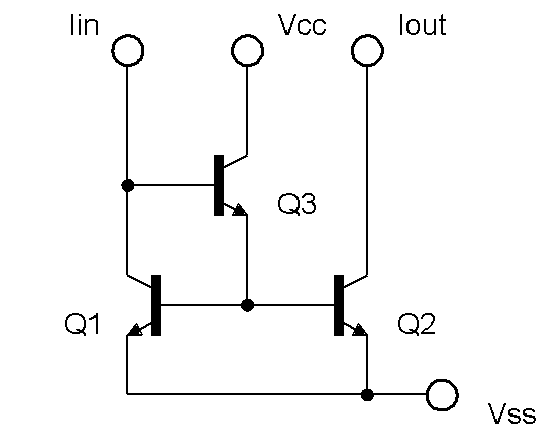
\includegraphics[scale=0.5]{obrazky/ZlepseneWilsonovoZrcadloNPN}
%   \end{center}
%   \caption[Alenčino zrcadlo]{Zlepšené Wilsonovo proudové zrcadlo.}
% \end{figure}

% Pro sazbu vektorových obrázků přímo v~\LaTeX{}u je možné doporučit balíček \href{https://www.ctan.org/pkg/pgf}{\texttt{TikZ}}.
% Příklady sazby je možné najít na \href{http://www.texample.net/tikz/examples/}{\TeX{}ample}.
% Pro vyzkoušení je možné použít programy QTikz nebo TikzEdt.




% \chapter{Příklad sazby zdrojových kódů}

% \section{Balíček \texttt{listings}}

% Pro vysázení zdrojových souborů je možné použít balíček \href{https://www.ctan.org/pkg/listings}{\texttt{listings}}.
% Balíček zavádí nové prostředí \texttt{lstlisting} pro sazbu zdrojových kódů, jako například:
% %
% \begin{lstlisting}[language={[LaTeX]TeX}]
% \section{Balíček lstlistings}
% Pro vysázení zdrojových souborů je možné použít
% 	balíček \href{https://www.ctan.org/pkg/listings}%
% 	{\texttt{listings}}.
% Balíček zavádí nové prostředí \texttt{lstlisting} pro
% 	sazbu zdrojových kódů.
% \end{lstlisting}
% %
% Podporuje množství programovacích jazyků.
% Kód k~vysázení může být načítán přímo ze zdrojových souborů.
% Umožňuje vkládat čísla řádků nebo vypisovat jen vybrané úseky kódu.
% Např.:

% \noindent
% Zkratky jsou sázeny v~prostředí \texttt{acronym}:
% \label{lst:zkratky}
% \lstinputlisting[language={[LaTeX]TeX},nolol,numbers=left, firstnumber=6, firstline=6,lastline=6]{text/zkratky.tex}
% %
% Šířka textu volitelného parametru \verb|KolikMista| udává šířku prvního sloupce se zkratkami.
% Proto by měla být zadávána nejdelší zkratka nebo symbol.
% Příklad definice zkratky \acs{symfvz} je na výpisu \ref{lst:symfvz}.

% \shorthandoff{-}
% \lstinputlisting[language={[LaTeX]TeX},frame=single,caption={Ukázka sazby zkratek},label=lst:symfvz,numbers=left,linerange={bsymfvz-\%\%\%\ esymfvz},includerangemarker=false]{text/zkratky.tex}
% \shorthandon{-}

% \noindent
% Ukončení seznamu je provedeno ukončením prostředí:
% \lstinputlisting[language={[LaTeX]TeX},nolol,numbers=left,firstnumber=26,linerange=26]{text/zkratky.tex}

% \vspace{\fill}

% \noindent
% {\bf Poznámka k~výpisům s~použitím volby jazyka \verb|czech| nebo \verb|slovak|:}\newline
% Pokud Váš zdrojový kód obsahuje znak spojovníku \verb|-|, pak překlad může skončit chybou.
% Ta je způsobená tím, že znak \verb|-| je v~českém nebo slovenském nastavení balíčku \verb|babel| tzv.\ aktivním znakem.
% Přepněte znak \verb|-| na neaktivní příkazem \verb|\shorthandoff{-}| těsně před výpisem a hned za ním jej vraťte na aktivní příkazem \verb|\shorthandon{-}|.
% Podobně jako to je ukázáno ve zdrojovém kódu šablony.


% \clearpage

% %\section{Výpis kódu prostředí Matlab}
% Na výpisu \ref{lst:priklad.vypis.kodu.Matlab} naleznete příklad kódu pro Matlab, na výpisu \ref{lst:priklad.vypis.kodu.C} zase pro jazyk~C.

% \lstnewenvironment{matlab}[1][]{%
% \iflanguage{czech}{\shorthandoff{-}}{}%
% \iflanguage{slovak}{\shorthandoff{-}}{}%
% \lstset{language=Matlab,numbers=left,#1}%
% }{%
% \iflanguage{slovak}{\shorthandon{-}}{}%
% \iflanguage{czech}{\shorthandon{-}}{}%
% }

% \begin{matlab}[frame=single,float=htbp,caption={Příklad Schur-Cohnova testu stability v~prostředí Matlab.},label=lst:priklad.vypis.kodu.Matlab,numberstyle=\scriptsize, numbersep=7pt]
% %% Priklad testovani stability filtru

% % koeficienty polynomu ve jmenovateli
% a = [ 5, 11.2, 5.44, -0.384, -2.3552, -1.2288];
% disp( 'Polynom:'); disp(poly2str( a, 'z'))

% disp('Kontrola pomoci korenu polynomu:');
% zx = roots( a);
% if( all( abs( zx) < 1))
%     disp('System je stabilni')
% else
%     disp('System je nestabilni nebo na mezi stability');
% end

% disp(' '); disp('Kontrola pomoci Schur-Cohn:');
% ma = zeros( length(a)-1,length(a));
% ma(1,:) = a/a(1);
% for( k = 1:length(a)-2)
%     aa = ma(k,1:end-k+1);
%     bb = fliplr( aa);
%     ma(k+1,1:end-k+1) = (aa-aa(end)*bb)/(1-aa(end)^2);
% end

% if( all( abs( diag( ma.'))))
%     disp('System je stabilni')
% else
%     disp('System je nestabilni nebo na mezi stability');
% end
% \end{matlab}

% \noindent
% \begin{minipage}{\linewidth}


% %\section{Výpis kódu jazyka C}

% \begin{lstlisting}[frame=single,numbers=right,caption={Příklad implementace první kanonické formy v~jazyce C.},label=lst:priklad.vypis.kodu.C,basicstyle=\ttfamily\small, keywordstyle=\color{black}\bfseries\underbar,]
% // první kanonická forma
% short fxdf2t( short coef[][5], short sample)
% {
% 	static int v1[SECTIONS] = {0,0},v2[SECTIONS] = {0,0};
% 	int x, y, accu;
% 	short k;

% 	x = sample;
% 	for( k = 0; k < SECTIONS; k++){
% 		accu = v1[k] >> 1;
% 		y = _sadd( accu, _smpy( coef[k][0], x));
% 		y = _sshl(y, 1) >> 16;

% 		accu = v2[k] >> 1;
% 		accu = _sadd( accu, _smpy( coef[k][1], x));
% 		accu = _sadd( accu, _smpy( coef[k][2], y));
% 		v1[k] = _sshl( accu, 1);

% 		accu = _smpy( coef[k][3], x);
% 		accu = _sadd( accu, _smpy( coef[k][4], y));
% 		v2[k] = _sshl( accu, 1);

% 		x = y;
% 	}
% 	return( y);
% }
% \end{lstlisting}
% \end{minipage}







% \chapter{Obsah elektronické přílohy}
% Elektronická příloha je často nedílnou součástí semestrální nebo závěrečné práce.
% Vkládá se do informačního systému VUT v~Brně ve vhodném formátu (ZIP, PDF\,\dots).

% Nezapomeňte uvést, co čtenář v~této příloze najde.
% Je vhodné okomentovat obsah každého adresáře, specifikovat, který soubor obsahuje důležitá nastavení, který soubor je určen ke spuštění, uvést nastavení kompilátoru atd.
% Také je dobře napsat, v~jaké verzi software byl kód testován (např.\ Matlab 2018b).
% Pokud bylo cílem práce vytvořit hardwarové zařízení,
% musí elektronická příloha obsahovat veškeré podklady pro výrobu (např.\ soubory s~návrhem DPS v~Eagle).

% Pokud je souborů hodně a jsou organizovány ve více složkách, je možné pro výpis adresářové struktury použít balíček \href{https://www.ctan.org/pkg/dirtree}{\texttt{dirtree}}.

% \bigskip

% {\small
% %
% \dirtree{%.
% .1 /\DTcomment{kořenový adresář přiloženého archivu}.
% .2 logo\DTcomment{loga školy a fakulty}.
% .3 BUT\_abbreviation\_color\_PANTONE\_EN.pdf.
% .3 BUT\_color\_PANTONE\_EN.pdf.
% .3 FEEC\_abbreviation\_color\_PANTONE\_EN.pdf.
% .3 FEKT\_zkratka\_barevne\_PANTONE\_CZ.pdf.
% .3 UTKO\_color\_PANTONE\_CZ.pdf.
% .3 UTKO\_color\_PANTONE\_EN.pdf.
% .3 VUT\_barevne\_PANTONE\_CZ.pdf.
% .3 VUT\_symbol\_barevne\_PANTONE\_CZ.pdf.
% .3 VUT\_zkratka\_barevne\_PANTONE\_CZ.pdf.
% .2 obrazky\DTcomment{ostatní obrázky}.
% .3 soucastky.png.
% .3 spoje.png.
% .3 ZlepseneWilsonovoZrcadloNPN.png.
% .3 ZlepseneWilsonovoZrcadloPNP.png.
% .2 pdf\DTcomment{pdf stránky generované informačním systémem}.
% .3 student-desky.pdf.
% .3 student-titulka.pdf.
% .3 student-zadani.pdf.
% .2 text\DTcomment{zdrojové textové soubory}.
% .3 literatura.tex.
% .3 prilohy.tex.
% .3 reseni.tex.
% .3 uvod.tex.
% .3 vysledky.tex.
% .3 zaver.tex.
% .3 zkratky.tex.
% %.2 navod-sablona\_FEKT.pdf\DTcomment{návod na používání šablony}.
% .2 sablona-obhaj.tex\DTcomment{hlavní soubor pro sazbu prezentace k~obhajobě}.
% %.2 readme.txt\DTcomment{soubor s~popisem obsahu CD}.
% .2 sablona-prace.tex\DTcomment{hlavní soubor pro sazbu kvalifikační práce}.
% .2 thesis.sty\DTcomment{balíček pro sazbu kvalifikačních prací}.
% }
% }


\end{document}